\section{SYSTEM CONTEXT PROCESSES \label{sec:system_context_processes}}

	\subsection{AGREEMENT PROCESSES\label{subsec:agreement_processes}}

	\begin{figure}[h]
		\centering
		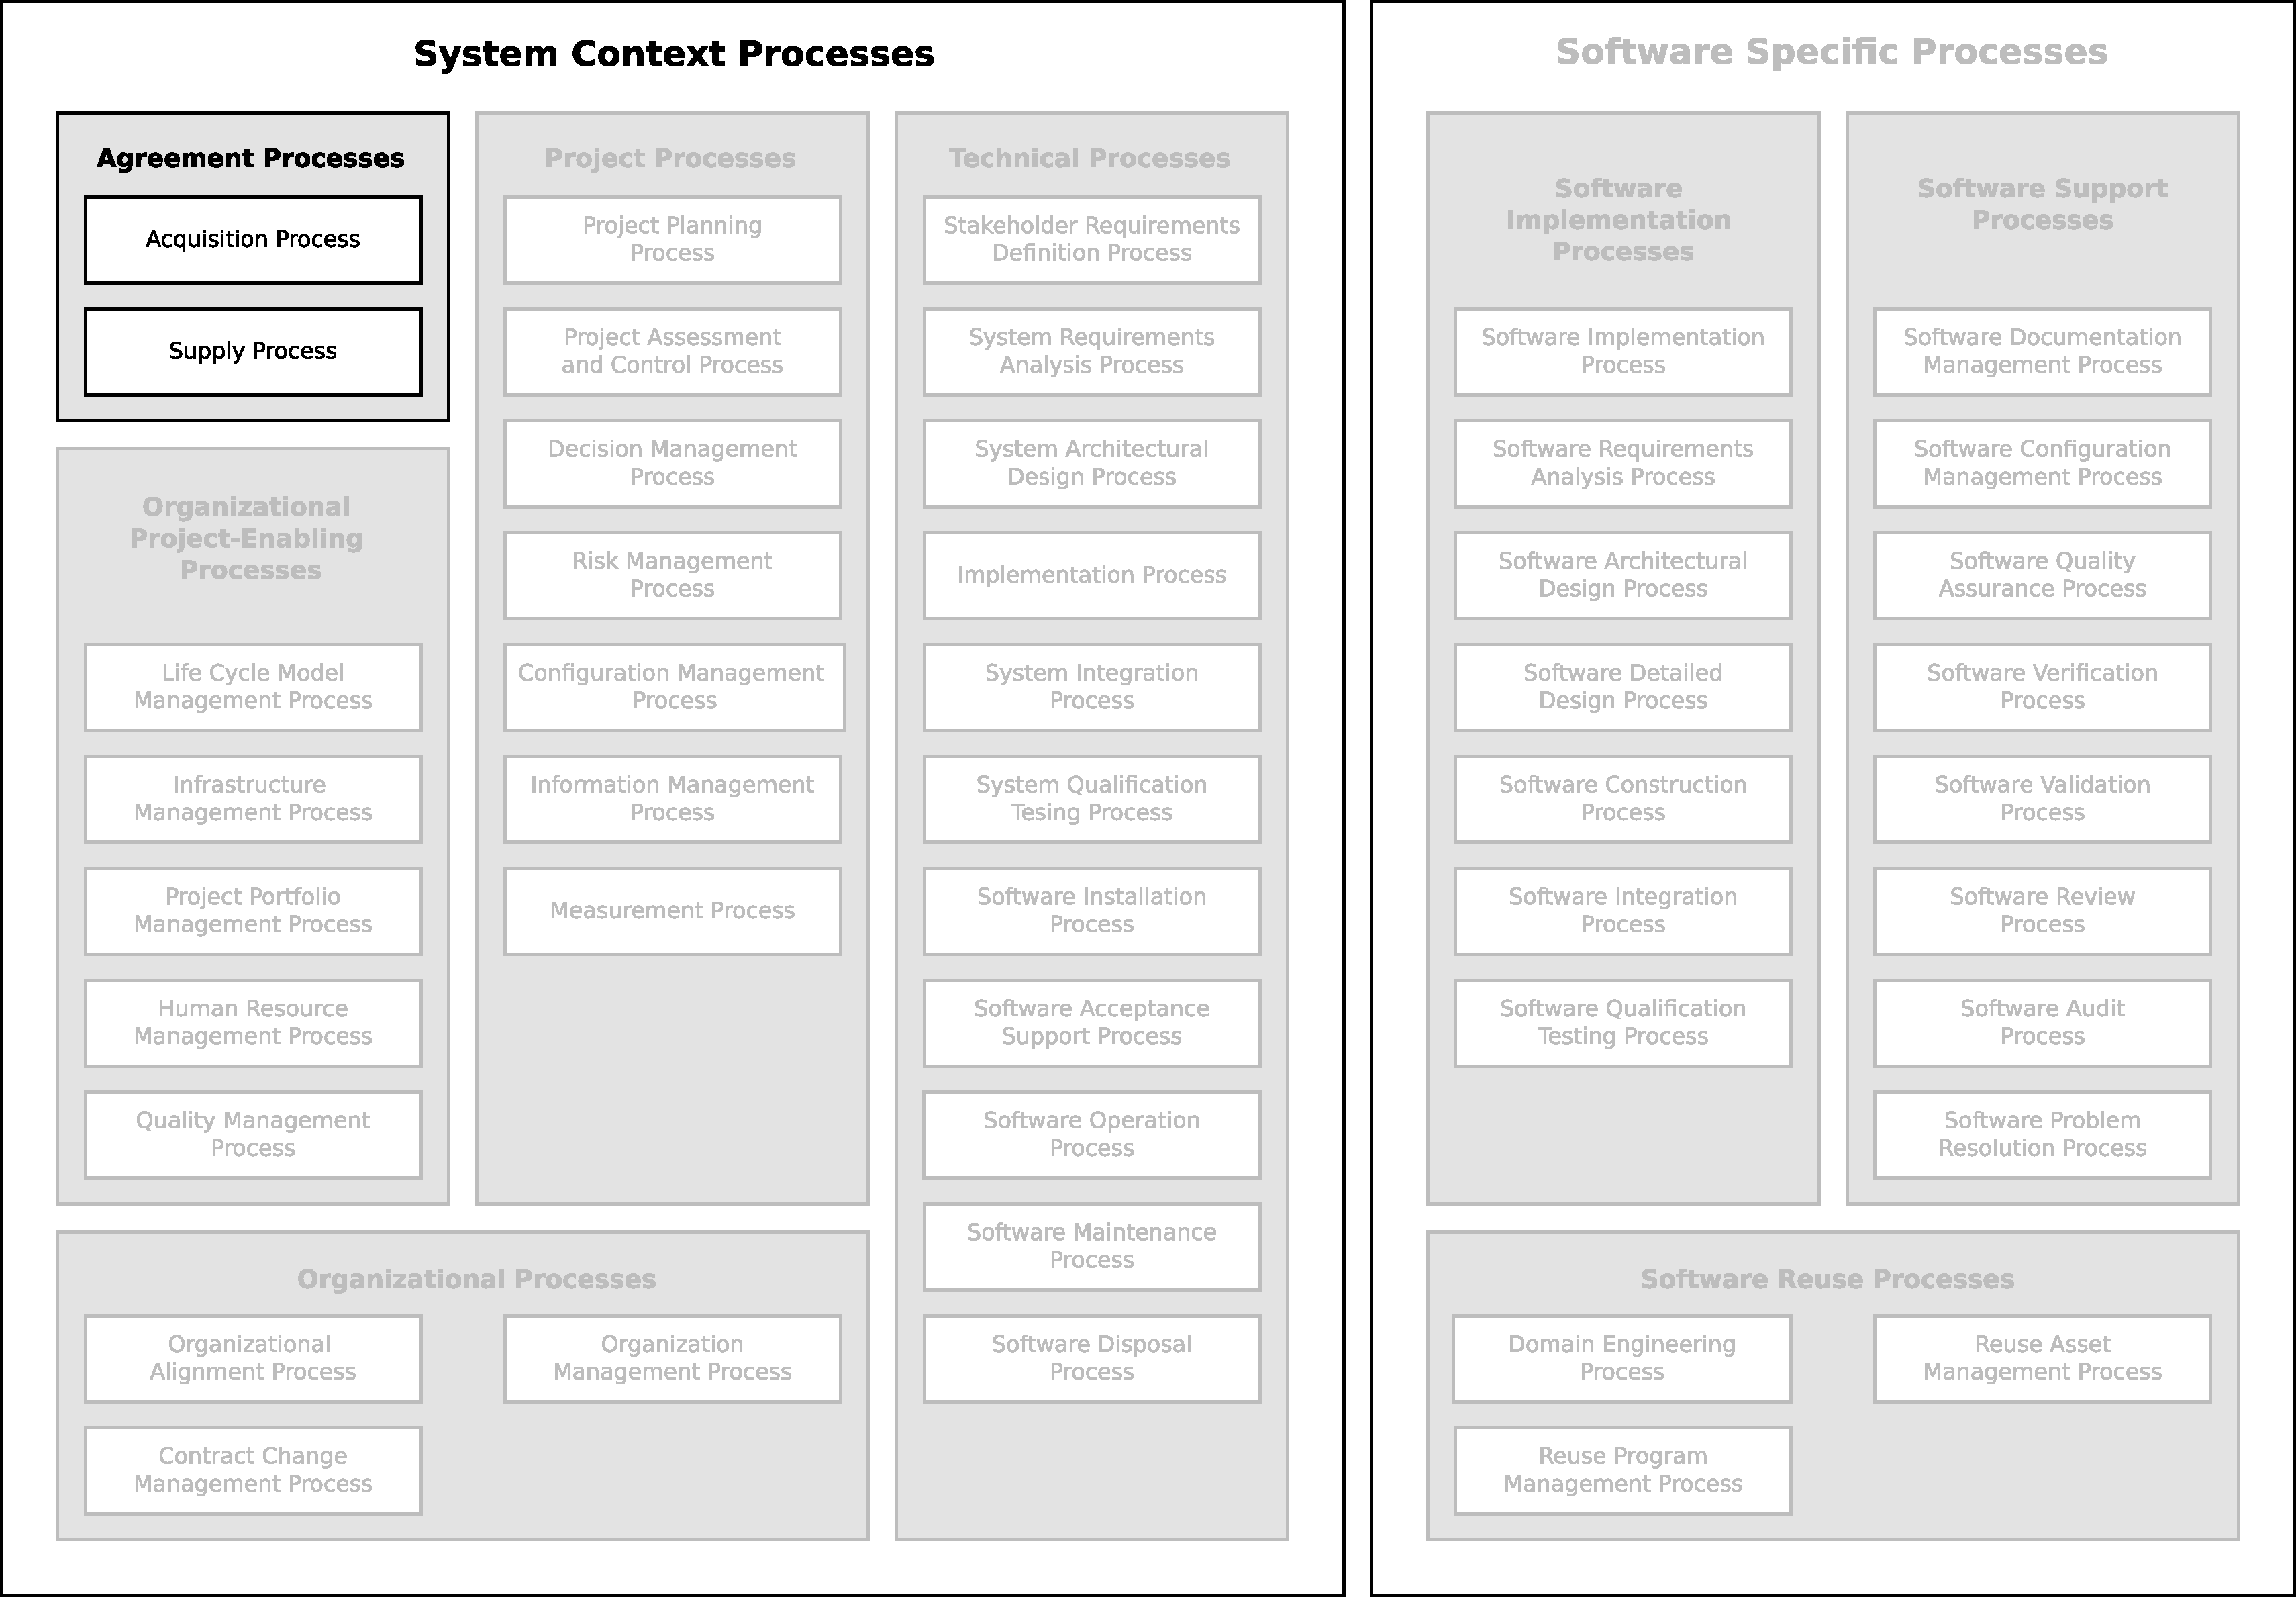
\includegraphics[width=15cm,keepaspectratio]{figures/life-cycle-process-groups-agreement-processes.pdf}
		\caption{Agreement Processes}
		\label{fig:agreement_processes}
	\end{figure}

	\begin{adjustwidth}{1em}{0pt}

		If the \nameref{proc:acquisition_process} is invoked, it provides the means for conducting business with a supplier of products that are supplied for use as an operational system, of services in support of an operational system, or of elements of a system being developed by a project. 

		If the \nameref{proc:supply_process} is invoked, it provides the means for conducting a project in which the result is a product or service that is delivered to the acquirer.

		In this Section:

		\begin{compactitem}
			\item \ref{proc:acquisition_process} - \nameref{proc:acquisition_process}
			\item \ref{proc:supply_process} - \nameref{proc:supply_process}
		\end{compactitem}

	\end{adjustwidth}

		\newpage
		\subsubsection{ACQUISITION PROCESS\label{proc:acquisition_process}}

			\subsubsubsection{PURPOSE}
			\begin{adjustwidth}{2em}{0pt}

				The purpose of the Acquisition Process is to obtain the product and/or service that satisfies the need expressed by the acquirer. The process begins with the identification of customer needs and ends with the acceptance of the product and/or service needed by the acquirer. 

			\end{adjustwidth}

			\subsubsubsection{OUTCOMES}
			\begin{adjustwidth}{2em}{0pt}

				\begin{compactitem}
					\item acquisition needs, goals, product and/or service acceptance criteria and acquisition strategies are defined;

					\item an agreement is developed that clearly expresses the expectation, responsibilities and liabilities of both the acquirer and the supplier;

					\item one or more suppliers is selected;

					\item a product and/or service is acquired that satisfies the acquirer's stated need
					
					\item the acquisition is monitored so that specified constraints such as cost, schedule and quality are met;
					
					\item supplier deliverables are accepted; and
					
					\item any identified open items have a satisfactory conclusion as agreed to by the acquirer and the supplier. 
				\end{compactitem}

			\end{adjustwidth}

			\subsubsubsection{ACTIVITIES AND TASKS}
			\begin{adjustwidth}{2em}{0pt}

				\begin{compactenum}

					\item {\bf Acquisition Preparation}

					\begin{compactenum}
						\item The acquirer begins the acquisition process by describing a concept or a need to acquire, develop, or enhance a system, software product or software service.

						\item The acquirer shall define and analyze the system requirements. The system requirements should include business, organizational and user as well as safety, security, and other criticality requirements along with related design, testing, and compliance standards and procedures.

						\item The acquirer may perform the definition and analysis of software requirements by itself or may retain a supplier to perform this task.

						\item If the acquirer retains a supplier to perform system or software requirements analysis, the acquirer shall retain approval authority for the analyzed requirements.

						\item The Technical Processes should be used to perform the tasks above. The acquirer may use the Stakeholder Requirements Definition Process to establish the customer requirements.

						\item The acquirer shall consider options for acquisition against analysis of appropriate criteria to include risk, cost and benefits for each option. Options include:

						\begin{compactitem}
							\item Purchase an off-the-shelf software product that satisfies the requirements.
							\item Develop the software product or obtain the software service internally.
							\item Develop the software product or obtain the software service through contract.
							\item A combination of the three items above.
							\item Enhance an existing software product or service.
						\end{compactitem}

						\item When an off-the-shelf software product is to be acquired, the acquirer shall ensure the following conditions are satisfied:

						\begin{compactitem}
							\item The requirements for the software product are satisfied.
							\item The required documentation is available.
							\item Proprietary, usage, ownership, warranty and licensing rights are satisfied.
							\item Future support for the software product is planned.
						\end{compactitem}

						\item The acquirer should prepare, document and execute an acquisition plan. The plan should contain the following:

						\begin{compactitem}
							\item Requirements for the system.
							\item Planned employment of the system.
							\item Type of contract to be employed.
							\item Responsibilities of the organizations involved.
							\item Support concept to be used.
							\item Risks considered as well as methods to manage the risks.
						\end{compactitem}

						\item The acquirer shall define and document the acceptance strategy and conditions (criteria).

						\item The acquirer should document the acquisition requirements (e.g., request for proposal), the content of which depends upon the acquisition option selected in previously defined task. The acquisition documentation should include, as appropriate:

						\begin{compactitem}
							\item System requirements.
							\item Scope statement.
							\item Instructions for bidders.
							\item List of software products.
							\item Terms and conditions.
							\item Control of subcontracts.
							\item Technical constraints (e.g. target environment).
						\end{compactitem}

						\item The acquirer should determine which processes of this standard are appropriate for the acquisition and specify any acquirer requirements for tailoring those processes. The acquirer should specify if any of the processes are to be performed by parties other than the supplier, so that suppliers may, in their proposals, define their approach to supporting the work of other parties. The acquirer shall define the scope of those tasks that reference the contract.

						\item The acquisition documentation shall also define the contract milestones at which the supplier's progress shall be reviewed and audited as part of monitoring the acquisition.

						\item The acquisition requirements should be given to the organization selected for performing the acquisition activities.
					\end{compactenum}

					\item {\bf Acquisition Advertisement}
					\begin{compactenum}
						\item The acquirer shall communicate the request for the supply of a product or service to identified suppliers. 
					\end{compactenum}

					\item {\bf Supplier Selection}
					\begin{compactenum}
						\item The acquirer should establish a procedure for supplier selection including proposal evaluation criteria and requirements compliance weighting.

						\item The acquirer should select a supplier based upon the evaluation of the suppliers' proposals, capabilities, and in accordance with the acquirer's acceptance strategy and conditions.
					\end{compactenum}

					\item {\bf Contract Agreement}
					\begin{compactenum}
						\item The acquirer may involve other parties, including potential suppliers or any necessary third parties (such as regulators), before contract award, in determining the acquirer's requirements for tailoring of this standard for the project. In making this determination, the acquirer shall consider the effect of the tailoring requirements upon the supplier's organizationally-adopted processes. The acquirer shall include or reference the tailoring requirements in the contract.

						\item The acquirer shall then prepare and negotiate a contract with the supplier that addresses the acquisition requirements, including the cost and schedule, of the software product or service to be delivered. The contract shall address proprietary, usage, ownership, warranty and licensing rights associated with the reusable off-the-shelf software products.

						\item Once the contract is underway, the acquirer shall control changes to the contract through negotiation with the supplier as part of a change control mechanism. Changes to the contract shall be investigated for impact on project plans, costs, benefits, quality, and schedule.
					\end{compactenum}

					\item {\bf Agreement Monitoring}
					\begin{compactenum}
						\item The acquirer shall monitor the supplier's activities in accordance with the Software Review Process and the Software Audit Process. The acquirer should supplement the monitoring with the Software Verification Process and the Software Validation Process as needed. 

						\item The acquirer shall cooperate with the supplier to provide all necessary information in a timely manner and resolve all pending items. 
					\end{compactenum}

					\item {\bf Acquirer Acceptance}
					\begin{compactenum}
						\item The acquirer should prepare for acceptance based on the defined acceptance strategy and criteria. The preparation of test cases, test data, test procedures, and test environment should be included. The extent of supplier involvement should be defined.

						\item The acquirer shall conduct acceptance review and acceptance testing of the deliverable software product or service and shall accept it from the supplier when all acceptance conditions are satisfied. The acceptance procedure should comply with the provisions defined by previous activities and tasks within this process.

						\item After acceptance, the acquirer should take the responsibility for the configuration management of the delivered software product
					\end{compactenum}

					\item {\bf Closure}
					\begin{compactenum}
						\item The acquirer shall make payment or provide other agreed consideration to the supplier for the product or service rendered.
					\end{compactenum}

				\end{compactenum}

			\end{adjustwidth}

		\newpage
		\subsubsection{SUPPLY PROCESS\label{proc:supply_process}}

			\subsubsubsection{PURPOSE}
			\begin{adjustwidth}{2em}{0pt}
				
				The purpose of the Supply Process is to provide a product or service to the acquirer that meets the agreed requirements.

			\end{adjustwidth}

			\subsubsubsection{OUTCOMES}
			\begin{adjustwidth}{2em}{0pt}

				\begin{compactitem}

					\item An acquirer for a product or service is identified;

					\item A response to an acquirer's request is produced;

					\item An agreement is established between the acquirer and the supplier for developing, maintaining, operating, packaging, delivering, and installing the product and/or service;

					\item A product and/or service that meets the agreed requirements are developed by the supplier;

					\item The product and/or service is delivered to the acquirer in accordance with the agreed requirements; and

					\item The product is installed in accordance with the agreed requirements.

				\end{compactitem}

			\end{adjustwidth}

			\subsubsubsection{ACTIVITIES AND TASKS}
			\begin{adjustwidth}{2em}{0pt}

				\begin{compactenum}

					\item {\bf Opportunity Identification}
					\begin{compactenum}

						\item The supplier should determine the existence and identity of an acquirer who has, or who represents an organization or organizations having, a need for a product or service.

					\end{compactenum}

					\item {\bf Supplier Tendering}
					\begin{compactenum}
						
						\item The supplier should conduct a review of requirements in the request for proposal taking into account organizational policies and other regulations.

						\item The supplier should make a decision to bid or accept the contract.

						\item The supplier shall prepare a proposal in response to the request for proposal.

					\end{compactenum}

					\item {\bf Contract Agreement}
					\begin{compactenum}

						\item The supplier shall negotiate and enter into a contract with the acquirer to provide the software product or service.

						\item The supplier may request modification to the contract as part of the change control mechanism.

					\end{compactenum}

					\item {\bf Contract Execution}
					\begin{compactenum}

						\item The supplier shall conduct a review of the acquisition requirements to define the framework for managing and assuring the project and for assuring the quality of the deliverable software product or service.

						\item If not stipulated in the contract, the supplier shall define or select a life cycle model appropriate to the scope, magnitude, and complexity of the project. The life cycle model shall be comprised of stages and the purpose and outcomes of each stage. The processes, activities, and tasks of this standard shall be selected and mapped onto the life cycle model.

						\item The supplier shall establish requirements for the plans for managing and assuring the project and for assuring the quality of the deliverable software product or service. Requirements for the plans should include resource needs and acquirer involvement.

						\item Once the planning requirements are established, the supplier shall consider the options for developing the software product or providing the software service against an analysis of risks associated with each option. Options include:

						\begin{compactenum}

							\item Develop the software product or provide the software service using internal resources.

							\item Develop the software product or provide the software service by subcontracting.

							\item Obtain off-the-shelf software products from internal or external sources.

							\item A combination of a, b, and c above.

						\end{compactenum}

						\item The supplier shall develop and document project management plan(s) based upon the planning requirements and options selected in previous point

						\begin{compactenum}

							\item Project organizational structure and authority and responsibility of each organizational unit, including external organizations.

							\item Engineering environment (for development, operation, or maintenance, as applicable), including test environment, library, equipment, facilities, standards, procedures, and tools.

							\item Work breakdown structure of the life cycle processes and activities, including the software products, software services and non-deliverable items, to be performed together with budgets, staffing, physical resources, software size, and schedules associated with the tasks.

							\item Management of the quality characteristics of the software products or services. Separate plans for quality may be developed.

							\item Management of the safety, security, and other critical requirements of the software products or services. Separate plans for safety and security may be developed.

							\item Subcontractor management, including subcontractor and the acquirer, if any. subcontractor selection and involvement between the subcontractor and the acquirer, if any. 

							\item Quality assurance.

							\item Verification and validation, including the approach for interfacing with the verification and validation agent, if specified. 

							\item Acquirer involvement; that is, by such means as reviews, audits, informal meetings, reporting, modification and change; implementation, approval, acceptance, and access to facilities.
							
							\item User involvement; by such means as requirements setting exercises, prototype demonstrations and evaluations.
							
							\item Risk management; that is, management of the areas of the project that involve potential technical, cost, or schedule risks.
							
							\item Security policy; that is, the rules for need-to-know and access-to-information at each project organization level.
							
							\item Approval required by such means as regulations, required certifications, proprietary, usage, ownership, warranty and licensing rights.
							
							\item Means for scheduling, tracking, and reporting.
							
							\item Training of personnel.

						\end{compactenum}

						\item The supplier shall implement and execute the project management plan(s) developed in previous point.

						\item The supplier shall:

						\begin{compactenum}

							\item Develop the software product in accordance with the Technical Processes
							
							\item Operate the software product in accordance with the Software Operation Process

							\item Maintain the software product in accordance with the Software Maintenance Process

						\end{compactenum}

						\item The supplier shall monitor and control the progress and the quality of the software products or services of the project throughout the contracted life cycle. This shall be an ongoing, iterative task, which shall provide for:

						\begin{compactenum}
							
							\item Monitoring progress of technical performance, costs, and schedules and reporting of project status.

							\item Problem identification, recording, analysis, and resolution.

						\end{compactenum}

						\item The supplier shall manage and control the subcontractors in accordance with the Acquisition Process. The supplier shall pass down all contractual requirements necessary to ensure that the software product or service delivered to the acquirer is developed or performed in accordance with the prime-contract requirements.
						
						\item The supplier shall interface with the independent verification, validation, or test agent as specified in the contract and project plans.

						\item The supplier shall interface with other parties as specified in the contract and project plans.

						\item The supplier should coordinate contract review activities, interfaces, and communication with the acquirer's organization.

						\item The supplier shall conduct or support the informal meetings, acceptance review, acceptance testing, joint reviews, and audits with the acquirer as specified in the contract and project plans. The joint reviews shall be conducted in accordance with the \nameref{proc:software_review_process}, audits in accordance with the \nameref{proc:software_audit_process}.

						\item The supplier should perform verification and validation in accordance with the \nameref{proc:software_verification_process} and \nameref{proc:software_validation_process} respectively to demonstrate that the software products or services and processes fully satisfy their respective requirements.

						\item The supplier shall make available to the acquirer the reports of evaluation, reviews, audits, testing, and problem resolutions as specified in the contract.

						\item The supplier shall provide the acquirer access to the supplier's and subcontractors' facilities for review of software products or services as specified in the contract and project plans.

						\item The supplier shall perform quality assurance activities in accordance with the \nameref{proc:software_quality_assurance_process}.

					\end{compactenum}

					\item {\bf Product/Service Delivery and Support}
					\begin{compactenum}

						\item The supplier shall deliver the software product or service as specified in the contract.

						\item The supplier shall provide assistance to the acquirer in support of the delivered software product or service as specified in the contract.

					\end{compactenum}

					\item {\bf Closure}:

					\begin{compactenum}

						\item The supplier shall accept and acknowledge payment or other agreed consideration.

						\item The supplier shall transfer the responsibility for the product or service to the acquirer, or other party, as directed by the agreement.

					\end{compactenum}

				\end{compactenum}

			\end{adjustwidth}


	\newpage 
	\subsection{ORGANIZATIONAL PROJECT-ENABLING PROCESSES\label{subsec:organizational_project_enabling_processes}}

		\begin{figure}[h]
			\centering
			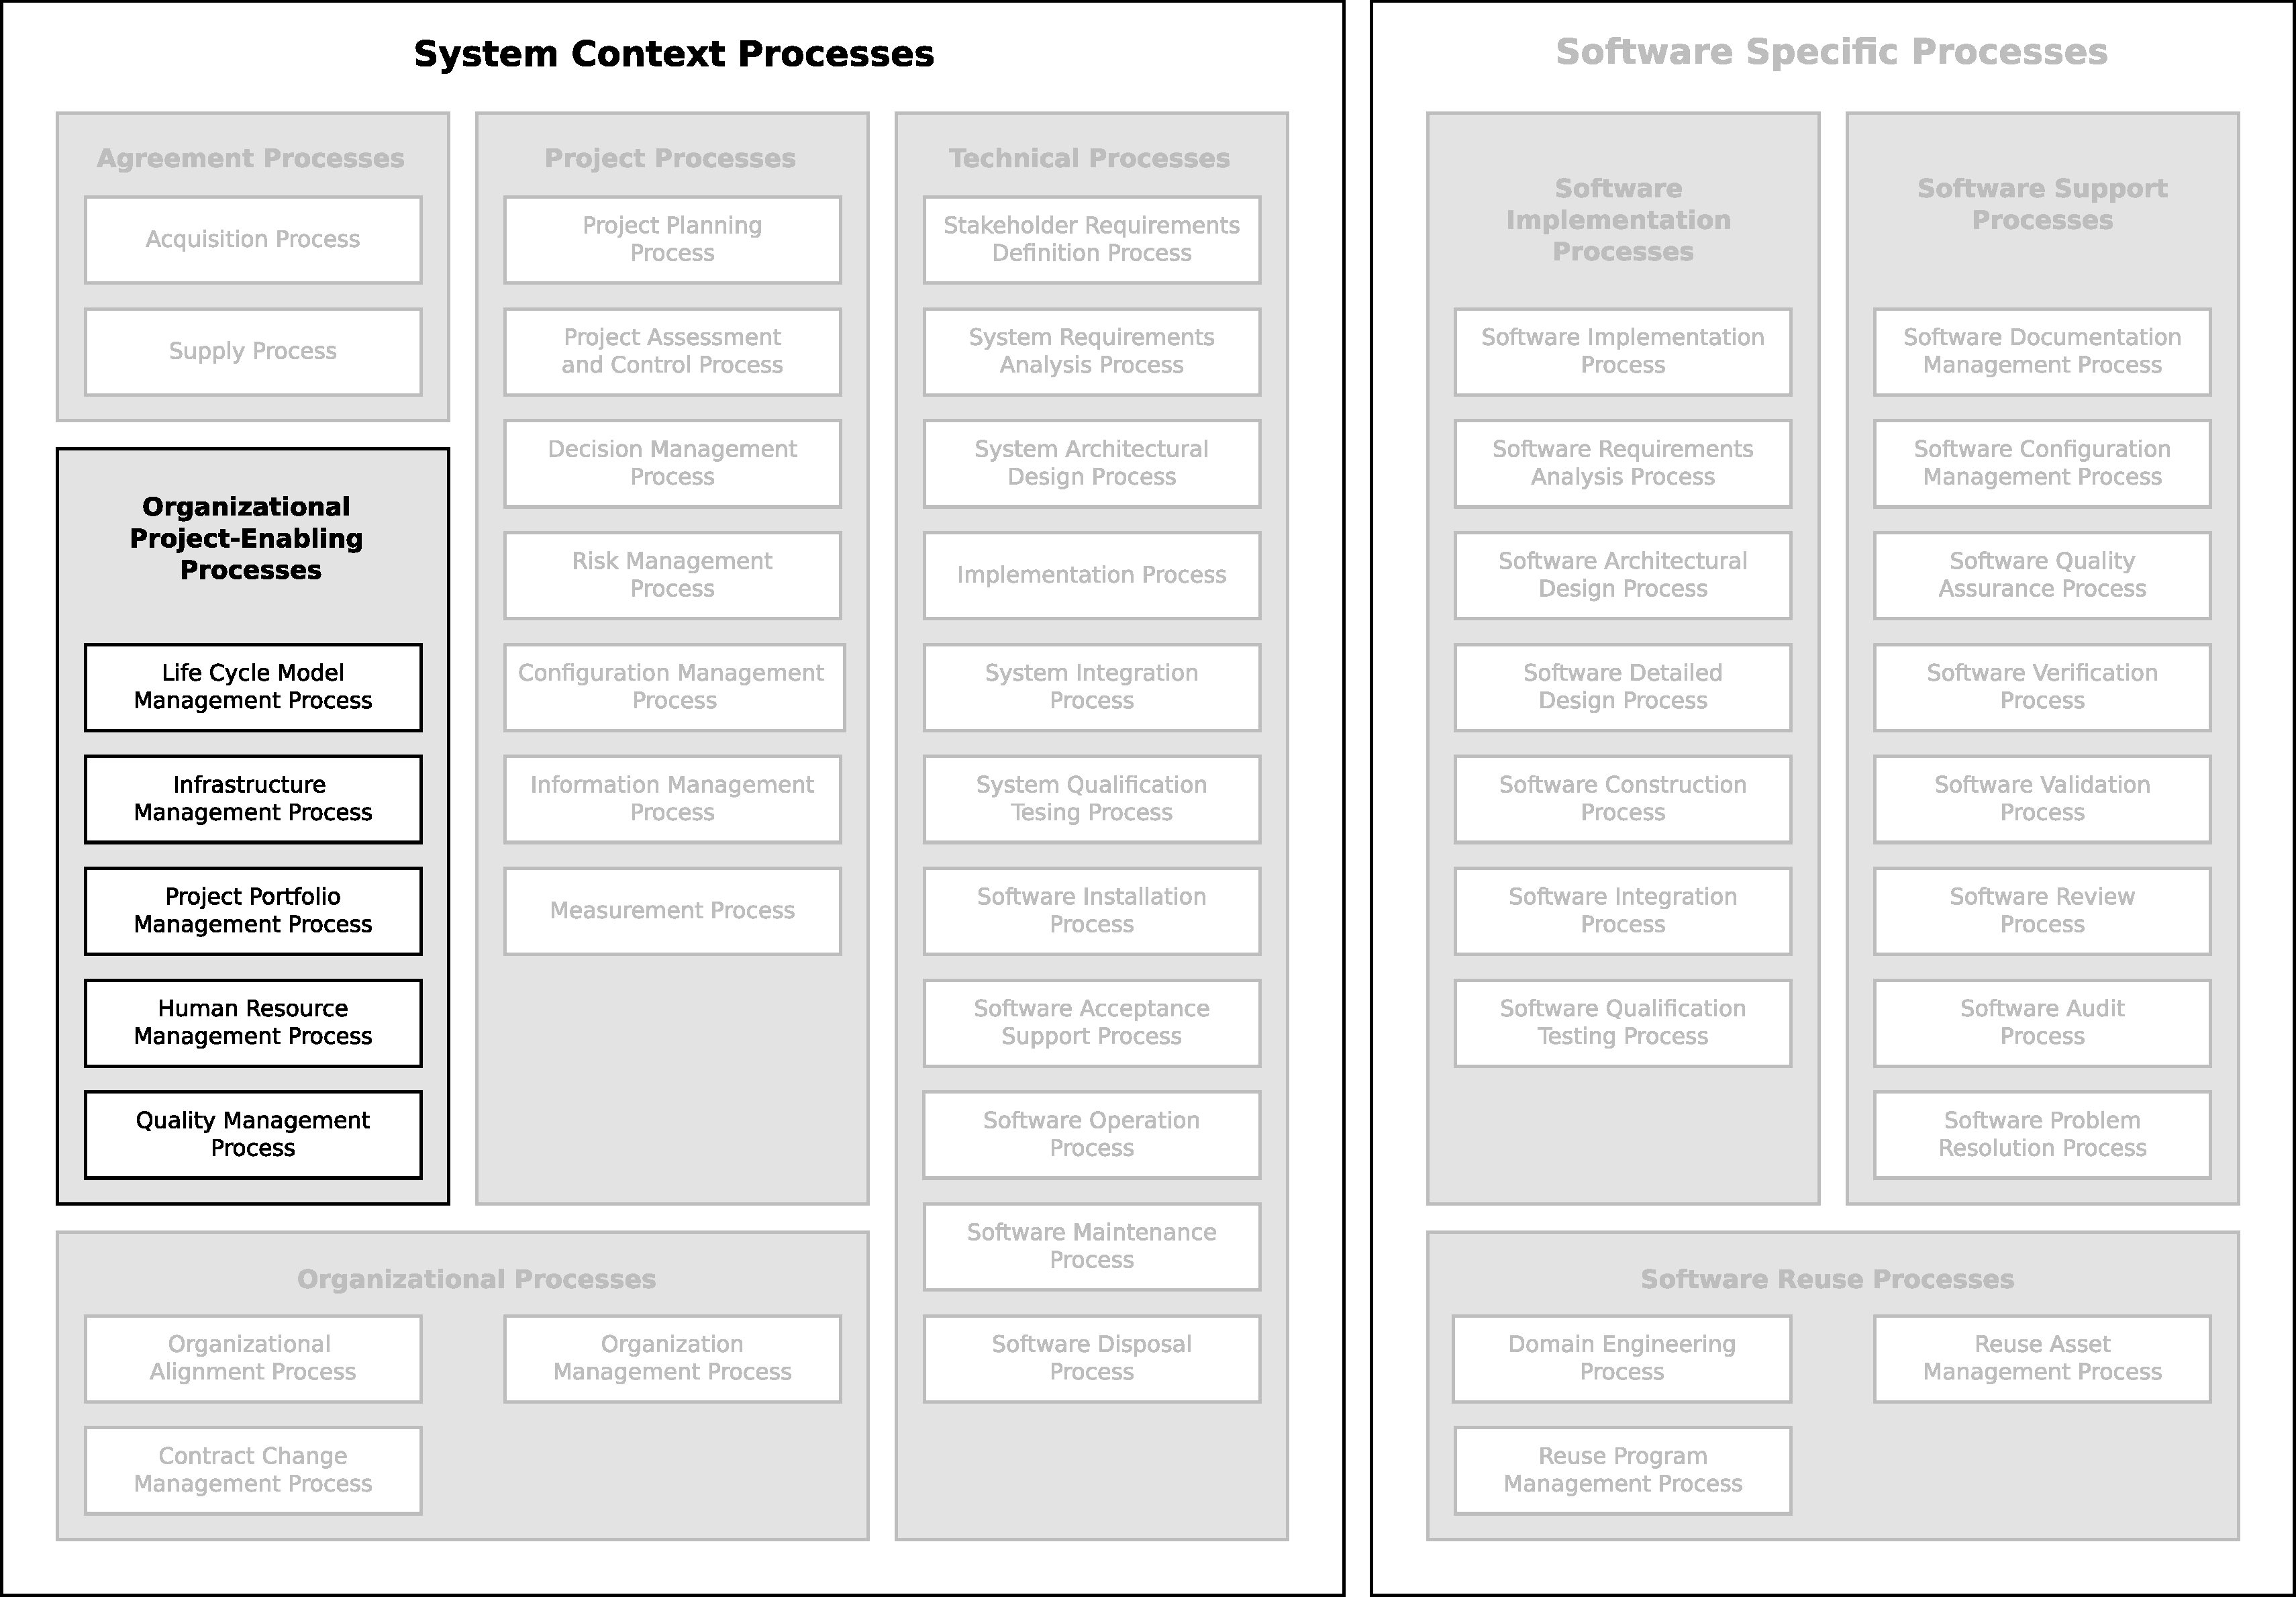
\includegraphics[width=15cm,keepaspectratio]{figures/life-cycle-process-groups-organizational-project-enabling-processes.pdf}
			\caption{Organizational Project-Enabling Processes}
			\label{fig:organizational_project_enabling_processes}
		\end{figure}

		\begin{adjustwidth}{1em}{0pt}

			The \nameref{subsec:organizational_project_enabling_processes} manage the organization's capability to acquire and supply products or services through the initiation, support and control of projects. 

			They provide resources and infrastructure necessary to support projects and ensure the satisfaction of organizational objectives and established agreements. They are not intended to be a comprehensive set of business processes that enable management of the organization's business.

			In this Section:

			\begin{compactitem}

				\item \ref{proc:life_cycle_model_management_process} - \nameref{proc:life_cycle_model_management_process}

				\item \ref{proc:infrastructure_management_process} - \nameref{proc:infrastructure_management_process}

				\item \ref{proc:project_portfolio_management_process} - \nameref{proc:project_portfolio_management_process}

				\item \ref{proc:human_resource_management_process} - \nameref{proc:human_resource_management_process}

				\item \ref{proc:quality_management_process} - \nameref{proc:quality_management_process}
			
			\end{compactitem}

		\end{adjustwidth}

		\newpage
		\subsubsection{LIFE CYCLE MODEL MANAGEMENT PROCESS\label{proc:life_cycle_model_management_process}}

			\subsubsubsection{PURPOSE}
			\begin{adjustwidth}{2em}{0pt} 

				The purpose of the Life Cycle Model Management Process is to define, maintain, and assure availability of policies, life cycle processes, life cycle models, and procedures for use by the organization with respect to the scope of this standard.

				This process provides life cycle policies, processes, and procedures that are consistent with the organization's objectives, that are defined, adapted, improved and maintained to support individual project needs within the context of the organization, and that are capable of being applied using effective, proven methods and tools.


			\end{adjustwidth}

			\subsubsubsection{OUTCOMES}
			\begin{adjustwidth}{2em}{0pt} 

				As a result of the successful implementation of the Life Cycle Model Management Process:

				\begin{compactitem}

					\item policies and procedures for the management and deployment of life cycle models and processes are provided;
					
					\item responsibility, accountability and authority for life cycle management are defined;
					
					\item life cycle processes, models and procedures for use by the organization are defined, maintained and improved; and
					
					\item prioritized process improvements are implemented.
				
				\end{compactitem}

			\end{adjustwidth}

			\subsubsubsection{ACTIVITIES AND TASKS}
			\begin{adjustwidth}{2em}{0pt} 

				\begin{compactenum}

					\item {\bf Process establishment}

					\begin{compactenum}

						\item The organization shall establish a suite of organizational processes for all software life cycle processes and life cycle models as they apply to its business activities. The processes and their application to specific cases shall be documented in the organization's publications. As appropriate, a process control mechanism should be established to develop, monitor, control, and improve the process(es).

					\end{compactenum}

					\item {\bf Process assessment}

					\begin{compactenum}

						\item The organization should develop, document and apply a process assessment procedure. Assessment records should be produced and maintained.

						\item The organization shall plan and carry out reviews of the processes at appropriate intervals to ensure their continuing suitability and effectiveness in the light of assessment results.

					\end{compactenum}

					\item {\bf Process improvement}

					\begin{compactenum}

						\item The organization shall effect such improvements to its processes as it determines to be necessary as a result of process assessment and review. Process documentation should be updated to reflect improvement in the organizational processes.
						
						\item Historical, technical, and evaluation data should be collected and analyzed to gain an understanding of the strengths and weaknesses of the employed processes. These analyses should be used as feedback to improve these processes, to recommend changes in the direction of the projects (or subsequent projects), and to determine technology advancement needs.

						\item Quality cost data should be collected, maintained, and used to improve the organization's processes as a management activity. These data shall serve the purpose of establishing the cost of both the prevention and resolution of problems and non-conformity in software products and services.
					
					\end{compactenum}

				\end{compactenum}

			\end{adjustwidth}
		
		\newpage
		\subsubsection{INFRASTRUCTURE MANAGEMENT PROCESS \label{proc:infrastructure_management_process}}

			\subsubsubsection{PURPOSE}
			\begin{adjustwidth}{2em}{0pt} 

				The purpose of the Infrastructure Management Process is to provide the enabling infrastructure and services to projects to support organization and project objectives throughout the life cycle.
				
				This process defines, provides and maintains the facilities, tools, and communications and information technology assets needed for the organization's business with respect to the scope of this standard.

			\end{adjustwidth}

			\subsubsubsection{OUTCOMES}
			\begin{adjustwidth}{2em}{0pt} 

				\begin{compactitem}

					\item The requirements for infrastructure to support processes are defined;

					\item The infrastructure elements are identified and specified;

					\item The infrastructure elements are implemented; and

					\item A stable and reliable infrastructure is maintained and improved.

				\end{compactitem}

				{\bf Note}: The infrastructure elements may include hardware, software, methods, tools, techniques, standards, and facilities for development, operation, or maintenance. 

			\end{adjustwidth}

			\subsubsubsection{ACTIVITIES AND TASKS}
			\begin{adjustwidth}{2em}{0pt} 

				The organization shall implement the following activities in accordance with applicable organization policies and procedures with respect to the \nameref{proc:infrastructure_management_process}.

				\begin{compactenum}

					\item {\bf Process implementation}:

					\begin{compactenum}
						
						\item The infrastructure should be defined and documented to meet the requirements of the process employing this process, considering the applicable procedures, standards, tools, and techniques.

						\item The establishment of the infrastructure should be planned and documented.

					\end{compactenum}

					\item {\bf Establishment of the infrastructure}:

					\begin{compactenum}
						
						\item The configuration of the infrastructure should be planned and documented. Functionality, performance, safety, security, availability, space requirements, equipment, costs, and time constraints should be considered.

						\item The infrastructure shall be installed in time for execution of the relevant process.

					\end{compactenum}

					\item {\bf Maintenance of the infrastructure}:

					\begin{compactenum}
						
						\item The infrastructure shall be maintained, monitored, and modified as necessary to ensure that it continues to satisfy the requirements of the process employing this process. As part of maintaining the infrastructure, the extent to which the infrastructure is under configuration management shall be defined.

					\end{compactenum}

				\end{compactenum}

			\end{adjustwidth}

		\newpage
		\subsubsection{PROJECT PORTFOLIO MANAGEMENT PROCESS\label{proc:project_portfolio_management_process}}

			\subsubsubsection{PURPOSE}
			\begin{adjustwidth}{2em}{0pt} 

				The purpose of the \nameref{proc:project_portfolio_management_process} is to initiate and sustain necessary, sufficient and suitable projects in order to meet the strategic objectives of the organization. 

				This process commits the investment of adequate organization funding and resources, and sanctions the authorities needed to establish selected projects. It performs continued qualification of projects to confirm they justify, or can be redirected to justify, continued investment.

			\end{adjustwidth}

			\subsubsubsection{OUTCOMES}
			\begin{adjustwidth}{2em}{0pt} 

				\begin{compactitem}

					\item Business venture opportunities, investments or necessities are qualified, prioritized and selected;

					\item Resources and budgets for each project are identified and allocated;

					\item Project management accountability and authorities are defined;

					\item Projects meeting agreement and stakeholder requirements are sustained; and

					\item projects not meeting agreement or stakeholder requirements are redirected or terminated.

				\end{compactitem}

			\end{adjustwidth}

			\subsubsubsection{ACTIVITIES AND TASKS}
			\begin{adjustwidth}{2em}{0pt} 
				
				The organization shall implement the following activities and tasks in accordance with applicable organization policies and procedures with respect to the \nameref{proc:project_portfolio_management_process}.

				\begin{compactenum}

					\item {\bf Project Initiation}:

					\begin{compactenum}

						\item The organization shall identify, prioritize, select, and establish new business opportunities, ventures, or undertakings in a manner that is consistent with the business strategy and action plans of the organization.

						\item The organization shall define accountabilities and authorities for each project.

						\item The organization shall identify the expected outcomes of the projects.

						\item The organization shall allocate resources for the achievement of project objectives.

						\item The organization shall identify any multi-project interfaces that must be managed or supported by the project.

						\item The organization shall specify the project reporting requirements and review milestones that will govern the execution of the project.
						
						\item The organization shall authorize the project to commence execution of approved project plans, including the technical plans.

					\end{compactenum}

					\item {\bf Project Evaluation}:

					\begin{compactenum}

						\item The organization shall evaluate ongoing projects to confirm that:

						\begin{compactenum}

							\item Projects are making progress towards achieving established goals.

							\item Projects are complying with project directives.

							\item Projects are being conducted according to system life cycle plans and procedures.

							\item Projects remain viable, as indicated by, for example, continuing need for the service, practicable product implementation, acceptable investment benefits.

						\end{compactenum}

						\item The organization shall act to continue or redirect projects that are satisfactorily progressing or can be expected to progress satisfactorily by appropriate redirection

					\end{compactenum}


					\item {\bf Project Closure}:

					\begin{compactenum}

						\item The organization shall act to cancel or suspend projects whose disadvantages or risks to the organization outweigh the benefits of continued investments, where agreements permit this.

						\item After completion of the agreement for products and services, the organization shall act to close the project per organizational policies and procedures and the agreement.

					\end{compactenum}

				\end{compactenum}

			\end{adjustwidth}

		\newpage
		\subsubsection{HUMAN RESOURCE MANAGEMENT PROCESS\label{proc:human_resource_management_process}}

			\subsubsubsection{PURPOSE}
			\begin{adjustwidth}{2em}{0pt} 
				
				The purpose of the \nameref{proc:human_resource_management_process} is to provide the organization with necessary human resources and to maintain their competencies, consistent with business needs. 

				The process assures the providing of a supply of skilled and experienced personnel qualified to perform life cycle processes to achieve organization, project and customer objectives.

			\end{adjustwidth}

			\subsubsubsection{OUTCOMES}
			\begin{adjustwidth}{2em}{0pt} 

				\begin{compactitem}

					\item skills required by projects are identified;

					\item necessary human resources are provided to projects;

					\item skills of personnel are developed, maintained or enhanced;

					\item conflicts in multi-project resource demands are resolved; and

					\item individual knowledge, information and skills are collected, shared, reused and improved throughout the organization.

				\end{compactitem}

			\end{adjustwidth}

			\subsubsubsection{ACTIVITIES AND TASKS}
			\begin{adjustwidth}{2em}{0pt} 

				\begin{compactenum}

					\item {\bf Skill Identification}

					\begin{compactenum}
						
						\item A review of the organization and project requirements shall be conducted to establish and make timely provision for acquiring or developing the resources and skills required by the management and technical staff. These needs may be met through training, recruitment or other staff development mechanisms.
						
						\item The types and levels of training and knowledge needed to satisfy organization and project requirements shall be determined.

					\end{compactenum}

					\item {\bf Skill Development}

					\begin{compactenum}
						
						\item A training plan, addressing implementation schedules, resource requirements, and training needs, should be developed and documented.

						\item Training manuals, including presentation materials used in providing training should be developed or acquired.
						
						\item The training plan shall be implemented to provide training to personnel. Training records should be maintained.

					\end{compactenum}

					\item {\bf Skill Acquisition and Provision}

					\begin{compactenum}
						
						\item Establish a systematic program for recruitment of staff qualified to meet the needs of the organization and projects. Provide opportunities for the career development of existing staff.

						\item Define objective criteria that can be used to evaluate staff performance.

						\item Evaluate the performance of the staff in respect of their contributions to the goals of the organization or project.

						\item Ensure that feedback is provided to the staff on the results of any evaluations performed.

						\item Maintain adequate records of staff performance including information on skills, training completed, and performance evaluations. 

						\item Define the organization's and project's need for project teams. Define team structure and operating rules.

						\item Conflicts in multi-project resource demands should be resolved.

						\item An understanding of their role on the project.

						\item A shared vision or sense of common interests on the success of the project.

						\item Appropriate mechanisms or facilities for communication and interactions among teams.

						\item Support from appropriate management to accomplish project requirements.

						\item It should be ensured that the right mix and categories of appropriately trained personnel are available for the planned activities and tasks in a timely manner.

					\end{compactenum}

					\item {\bf Knowledge Management}

					\begin{compactenum}	

						\item The organization shall plan the requirements for managing the organization's knowledge assets. The planning shall  include the definition of the infrastructure and training to support the contributors and the users of the organization's knowledge assets, the classification schema for the assets and the asset criteria.
						
						\item The organization shall establish a network of experts within the organization. The network shall contain the identification of the organization's experts, a list of their area of expertise and the identification of available information within a classification schema, e.g., knowledge area. The organization shall ensure that the network is maintained current.

						\item The organization shall establish a mechanism to support the exchange of information between the experts and the flow of expert information to the organization's projects. The mechanism shall support the organization's access, storage and retrieval requirements.

						\item The organization shall perform configuration management of assets in accordance with the \nameref{proc:configuration_management_process}.

						\item The organizations shall capture and maintain information for access by the organization per the plan.

					\end{compactenum}

				\end{compactenum}

			\end{adjustwidth}

		\newpage
		\subsubsection{QUALITY MANAGEMENT PROCESS\label{proc:quality_management_process}}

			\subsubsubsection{PURPOSE}
			\begin{adjustwidth}{2em}{0pt} 
				
				The purpose of the \nameref{proc:quality_management_process} is to assure that products, services and implementations of life cycle processes meet organizational quality objectives and achieve customer satisfaction.

			\end{adjustwidth}

			\subsubsubsection{OUTCOMES}
			\begin{adjustwidth}{2em}{0pt} 

				\begin{compactitem}

					\item organization quality management policies and procedures are defined;

					\item organization quality objectives are defined;

					\item accountability and authority for quality management are defined;

					\item the status of customer satisfaction is monitored; and

					\item appropriate action is taken when quality objectives are not achieved.

				\end{compactitem}

			\end{adjustwidth}

			\subsubsubsection{ACTIVITIES AND TASKS}
			\begin{adjustwidth}{2em}{0pt} 

				\begin{compactenum}

					\item {\bf Quality Management}

					\begin{compactenum}
						
						\item The organization shall establish quality management policies, standards and procedures.

						\item The organization shall establish organization quality management goals and objectives based on business strategy for customer satisfaction.
						
						\item The organization shall define responsibilities and authority for implementation of quality management.

						\item The organization shall assess customer satisfaction and report.

						\item The organization shall conduct periodic reviews of project quality plans.

						\item The organization shall monitor the status of quality improvements on products and services.

					\end{compactenum}


					\item {\bf Quality Management Corrective Action}

					\begin{compactenum}

						\item The organization shall take corrective actions when quality management goals are not
						
						\item The organization shall implement corrective actions and communicate results through the organization.

					\end{compactenum}

				\end{compactenum}

			\end{adjustwidth}


	\newpage 
	\subsection{PROJECT PROCESSES\label{subsec:project_processes}}

		\begin{figure}[h]
			\centering
			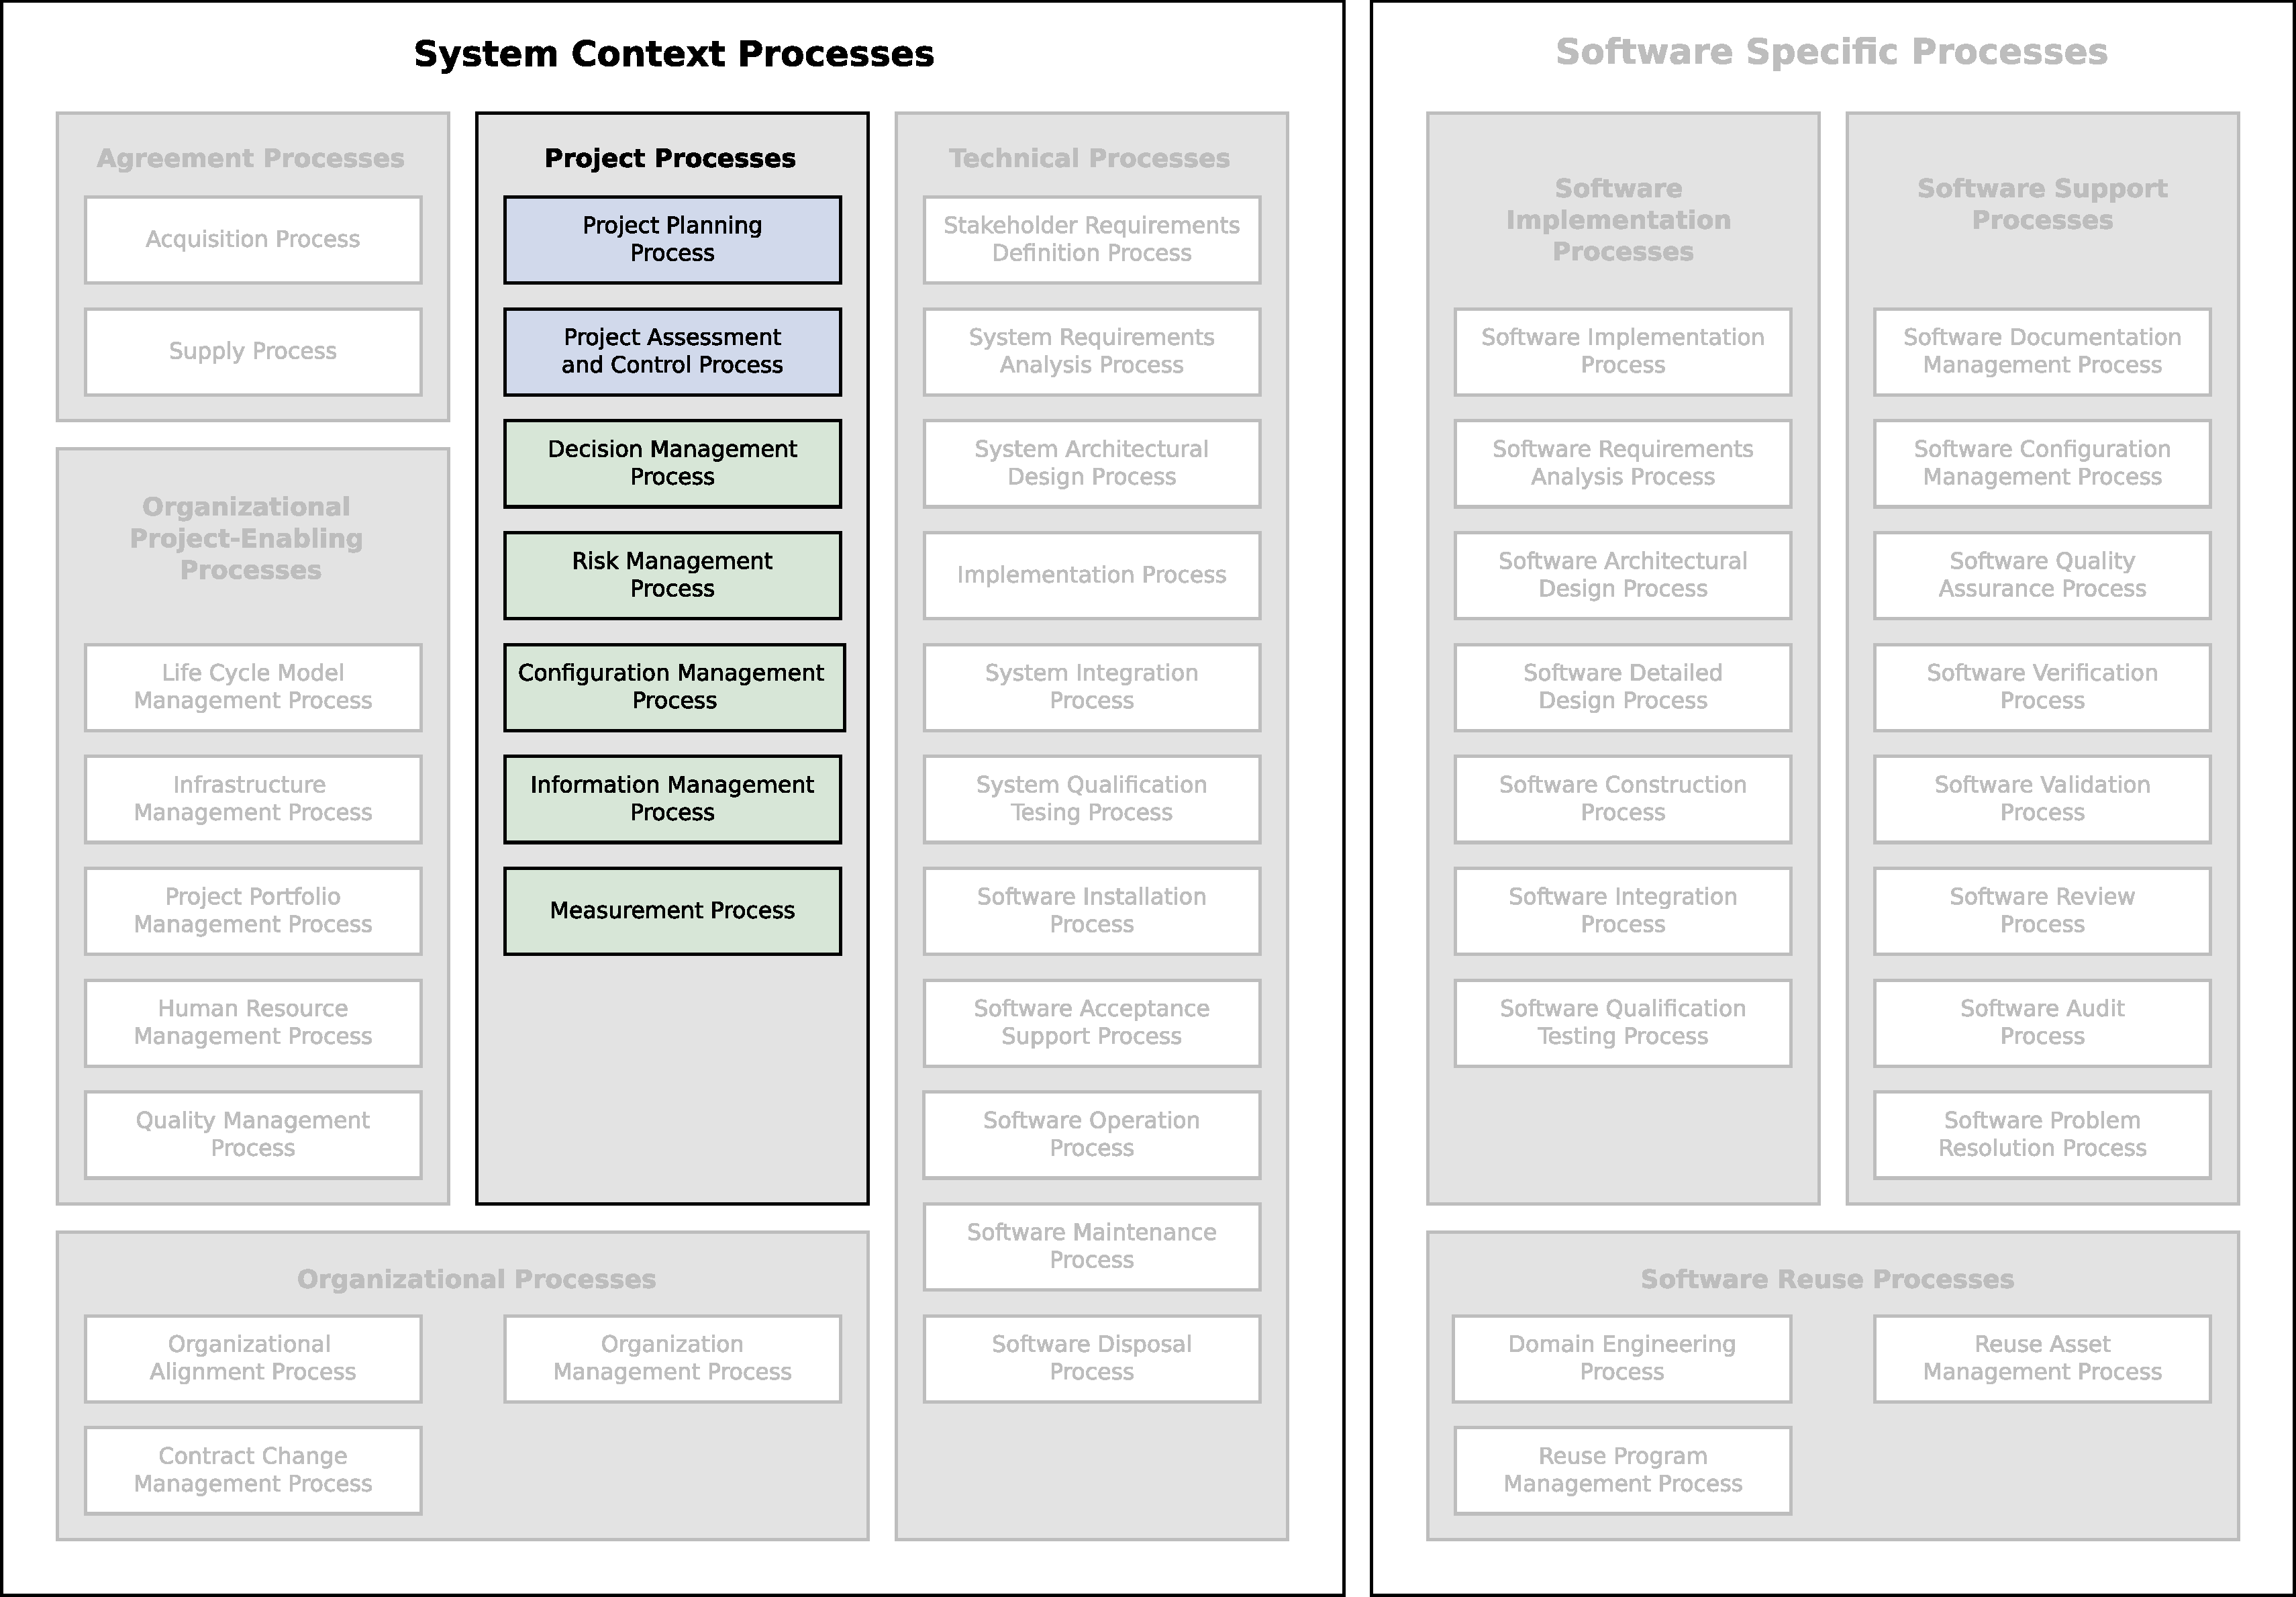
\includegraphics[width=15cm,keepaspectratio]{figures/life-cycle-process-groups-project-processes.pdf}
			\caption{Project Processes}
			\label{fig:project_processes}
		\end{figure}

		\begin{adjustwidth}{1em}{0pt}

			Within this standard, the project has been chosen as the context for describing processes concerned with planning, assessment and control. The principles related to these processes can be applied in any area of an organization's management.

			There are two categories of Project Processes. The Project Management Processes are used to plan, execute, assess and control the progress of a project. The Project Support Processes support specialized management objectives. Both are described below.
			
			The Project Management Processes are used to establish and evolve project plans, to assess actual achievement and progress against the plans and to control execution of the project through to fulfillment. Individual Project Management Processes may be invoked at any time in the life cycle and at any level in a hierarchy of projects, as required by project plans or unforeseen events. The Project Management Processes are applied with a level of rigor and formality that depends on the risk and complexity of the project.

			The Project Support Processes provide a specific focused set of tasks for performing a specialized management objective. They are all evident in the management of any undertaking, ranging from a complete organization down to a single life cycle process and its tasks.

		\end{adjustwidth}
		
		\newpage
		\subsubsection{PROJECT PLANNING PROCESS\label{proc:project_planning_process}}

			\subsubsubsection{PURPOSE}
			\begin{adjustwidth}{2em}{0pt}

				The purpose of the \nameref{proc:project_planning_process} is to produce and communicate effective and workable project plans.

				This process determines the scope of the project management and technical activities, identifies process outputs, project tasks and deliverables, establishes schedules for project task conduct, including achievement criteria, and required resources to accomplish project tasks.

			\end{adjustwidth}

			\subsubsubsection{OUTCOMES}
			\begin{adjustwidth}{2em}{0pt}

				\begin{compactitem}
					\item The scope of the work for the project is defined;
					\item The feasibility of achieving the goals of the project with available resources and constraints are evaluated;
					\item The tasks and resources necessary to complete the work are sized and estimated;
					\item Interfaces between elements in the project, and with other project and organizational units, are identified;
					\item Plans for the execution of the project are developed; and
					\item Plans for the execution of the project are activated.
				\end{compactitem}
			
			\end{adjustwidth}

			\subsubsubsection{ACTIVITIES AND TASKS}
			\begin{adjustwidth}{2em}{0pt}

				\begin{compactenum}

					\item {\bf Project initiation}:
					\begin{compactenum}
						\item The manager shall establish the requirements of the project to be undertaken.

						\item Once the project requirements are established, the manager shall establish the feasibility of the project by checking that the resources (personnel, materials, technology, and environment) required to execute and manage the project are available, adequate, and appropriate and that the timescales to completion are achievable.

						\item As necessary, and by agreement of all parties concerned, the requirements of the project may be modified at this point to achieve the completion criteria.
					\end{compactenum}

					\item {\bf Project planning}:
					\begin{compactenum}
						\item The manager shall prepare the plans for execution of the project. The plans associated with the execution of the project shall contain descriptions of the associated activities and tasks and identification of the software products that will be provided. These plans shall include, but are not limited to, the following:

						\begin{compactenum}
							\item Schedules for the timely completion of tasks.
							\item Estimation of effort.
							\item Adequate resources needed to execute the tasks.
							\item Allocation of tasks.
							\item Assignment of responsibilities.
							\item Quantification of risks associated with the tasks or the process itself.
							\item Quality assurance measures to be employed throughout the project.
							\item Costs associated with the process execution.
							\item Provision of environment and infrastructure.
							\item Definition and maintenance of a life cycle model that is comprised of stages using the defined life cycle models for projects of the organization
						\end{compactenum}

					\end{compactenum}

					\item {\bf Project activation}:
					\begin{compactenum}
						\item The manager shall obtain authorization for the project.

						\item The manager shall submit requests for necessary resources to perform the project.

						\item The manager shall initiate the implementation of the project plan/s to satisfy the objectives and criteria set, exercising control over the project
					\end{compactenum}

				\end{compactenum}

			\end{adjustwidth}

		\newpage
		\subsubsection{PROJECT ASSESSMENT AND CONTROL PROCESS\label{proc:project_assessment_and_control_process}}

			\subsubsubsection{PURPOSE}
			\begin{adjustwidth}{2em}{0pt}

				The purpose of the \nameref{proc:project_assessment_and_control_process} is to determine the status of the project and ensure that the project performs according to plans and schedules, and within projected budgets, and that it satisfies technical objectives. 

				This process includes redirecting the project activities, as appropriate, to correct identified deviations and variations from other project management or technical processes. Redirection may include replanning as appropriate.
			
			\end{adjustwidth}

			\subsubsubsection{OUTCOMES}
			\begin{adjustwidth}{2em}{0pt}

				\begin{compactitem}

					\item progress of the project is monitored and reported;

					\item interfaces between elements in the project, and with other project and organizational units, are monitored;

					\item actions to correct deviations from the plan and to prevent recurrence of problems identified in the project are taken when project targets are not achieved; and

					\item project objectives are achieved and recorded.

				\end{compactitem}

			\end{adjustwidth}

			\subsubsubsection{ACTIVITIES AND TASKS}
			\begin{adjustwidth}{2em}{0pt} 

				\begin{compactenum}

					\item {\bf Project Monitoring}

					\begin{compactenum}

						\item The manager shall monitor the overall execution of the project, providing both internal reporting of the project progress and external reporting to the acquirer as defined in the contract.

					\end{compactenum}


					\item {\bf Project Control}

					\begin{compactenum}
						
						\item The manager shall investigate, analyze, and resolve the problems discovered during the execution of the project. The resolution of problems may result in changes to plans. It is the manager's responsibility to ensure the impact of any changes is determined, controlled, and monitored. Problems and their resolution shall be documented.

						\item The manager shall report, at agreed points, the progress of the project, declaring adherence to the plans and resolving instances of the lack of progress. These include internal and external reporting as required by the organizational procedures and the contract.

					\end{compactenum}

					\item {\bf Project Assessment}

					\begin{compactenum}

						\item The manager shall ensure that the software products and plans are evaluated for satisfaction of requirements.

						\item The manager shall assess the evaluation results of the software products, activities, and tasks completed during the execution of the project for achievement of the objectives and completion of the plans.

					\end{compactenum}


					\item {\bf Project Closure}

					\begin{compactenum}

						\item When all software products, activities, and tasks are completed, the manager shall determine whether the project is complete, taking into account the criteria as specified in the contract or as part of organization's procedure.

						\item These results and records shall be archived in a suitable environment as specified in the contract.

					\end{compactenum}

				\end{compactenum}

			\end{adjustwidth}

		\newpage
		\subsubsection{DECISION MANAGEMENT PROCESS\label{proc:decision_management_process}}

			\subsubsubsection{PURPOSE}
			\begin{adjustwidth}{2em}{0pt} 

				The purpose of the \nameref{proc:decision_management_process} is to select the most beneficial course of project action where alternatives exist.

				This process responds to a request for a decision encountered during the system life cycle, whatever its nature or source, in order to reach specified, desirable or optimized outcomes. Alternative actions are analyzed and a course of action selected and directed. Decisions and their rationale are recorded to support future decision-making.

			\end{adjustwidth}

			\subsubsubsection{OUTCOMES}
			\begin{adjustwidth}{2em}{0pt} 

				\begin{compactitem}

					\item a decision-making strategy is defined;

					\item alternative courses of action are defined;

					\item a preferred course of action is selected; and

					\item the resolution, decision rationale and assumptions are captured and reported. 

				\end{compactitem}

			\end{adjustwidth}

			\subsubsubsection{ACTIVITIES AND TASKS}
			\begin{adjustwidth}{2em}{0pt} 

				\begin{compactenum}

					\item {\bf Decision Planning}:
					\begin{compactenum}

						\item The project shall involve relevant parties in the decision-making in order to draw on experience and knowledge.

						\item The project shall identify the circumstances and need for a decision.

					\end{compactenum}

					\item {\bf Decision Analysis}:
					\begin{compactenum}

						\item The project shall select and declare the decision-making strategy for each decision situation. 

						\item The project shall identify desired outcomes and measurable success criteria.
						
						\item The project shall evaluate the balance of consequences of alternative actions, using the defined decision-making strategy, to arrive at an optimization of, or an improvement in, an identified decision situation.

					\end{compactenum}

					\item {\bf Decision Tracking}:
					\begin{compactenum}

						\item The project shall record, track, evaluate and report decision outcomes to confirm that problems have been effectively resolved, adverse trends have been reversed and advantage has been taken of opportunities.

						\item The project shall maintain records of problems and opportunities and their disposition, as stipulated in agreements or organizational procedures and in a manner that permits auditing and learning from experience.
						
					\end{compactenum}

				\end{compactenum}

			\end{adjustwidth}

		\newpage
		\subsubsection{RISK MANAGEMENT PROCESS\label{proc:risk_management_process}}

			\subsubsubsection{PURPOSE}
			\begin{adjustwidth}{2em}{0pt} 
				
				The purpose of the \nameref{proc:risk_management_process} is to identify, analyze, treat and monitor the risks continuously.

				The Risk Management Process is a continuous process for systematically addressing risk throughout the life cycle of a system or software product or service. It can be applied to risks related to the acquisition, development, maintenance or operation of a system.

			\end{adjustwidth}

			\subsubsubsection{OUTCOMES}
			\begin{adjustwidth}{2em}{0pt} 

				\begin{compactitem}

					\item the scope of risk management to be performed is determined;

					\item appropriate risk management strategies are defined and implemented;

					\item risks are identified as they develop and during the conduct of the project;

					\item risks are analyzed, and the priority in which to apply resources to treatment of these risks is determined;

					\item risk measures are defined, applied, and assessed to determine changes in the status of risk and the progress of the treatment activities; and

					\item appropriate treatment is taken to correct or avoid the impact of risk based on its priority, probability, and consequence or other defined risk threshold.

				\end{compactitem}

			\end{adjustwidth}

			\subsubsubsection{ACTIVITIES AND TASKS}
			\begin{adjustwidth}{2em}{0pt} 

				\begin{compactenum}

					\item {\bf Risk Management Planning}:

					\begin{compactenum}
						\item Risk management policies describing the guidelines under which risk management is to be performed shall be defined.

						\item A description of the Risk Management Process to be implemented shall be documented.

						\item The parties responsible for performing risk management and their roles and responsibilities shall be identified.

						\item The responsible parties shall be provided with adequate resources to perform the Risk Management Process.

						\item A description of the process for evaluating and improving the Risk Management Process shall be provided.
					\end{compactenum}

					\item {\bf Risk Profile Management}:

					\begin{compactenum}
						\item Risk thresholds, defining the conditions under which a level of risk may be accepted, shall be documented.

						\item A risk profile shall be established and maintained.

						\item The relevant risk profile shall be communicated periodically to stakeholders based upon their needs.
					\end{compactenum}

					\item {\bf Risk Analysis}:

					\begin{compactenum}
						\item Risks shall be identified in the categories described in the risk management context.

						\item The probability of occurrence and consequences of each risk identified shall be estimated.

						\item Each risk shall be evaluated against its risk thresholds.

						\item For each risk that is above its risk threshold, recommended treatment strategies shall be defined and documented. Measures indicating the effectiveness of the treatment alternatives shall also be defined and documented.

						\item Stakeholders shall be provided recommended alternatives for risk treatment in risk action requests.
					\end{compactenum}

					\item {\bf Risk Treatment}:

					\begin{compactenum}
						\item If the stakeholders determine that actions should be taken to make a risk acceptable, then a risk treatment alternative shall be implemented.

						\item If the stakeholders accept a risk that exceeds its threshold, it shall be considered a high priority and monitored continuously to determine if any future risk treatment actions are necessary.

						\item Once a risk treatment is selected, it shall receive the same management actions as problems do, in accordance with the assessment and control activities in the \nameref{proc:project_assessment_and_control_process}.
					\end{compactenum}

					\item {\bf Risk Monitoring}:

					\begin{compactenum}
						\item All risks and the risk management context shall be continuously monitored for changes. Risks whose states have changed shall undergo risk evaluation.

						\item Measures shall be implemented and monitored to evaluate the effectiveness of risk treatments.

						\item The project shall continuously monitor for new risks and sources throughout its life cycle.
					\end{compactenum}

					\item {\bf Risk Management Process Evaluation}:

					\begin{compactenum}
						\item Information shall be collected throughout the project's life cycle for purposes of improving the Risk Management Process and generating lessons learned.

						\item The Risk Management Process shall be periodically reviewed for its effectiveness and efficiency.

						\item Information on the risks identified, their treatment, and the success of the treatments shall be reviewed periodically for purposes of identifying systemic project and organizational risks.
					\end{compactenum}

				\end{compactenum}

			\end{adjustwidth}

		\newpage
		\subsubsection{CONFIGURATION MANAGEMENT PROCESS\label{proc:configuration_management_process}}

			\subsubsubsection{PURPOSE}
			\begin{adjustwidth}{2em}{0pt} 

				The purpose of the \nameref{proc:configuration_management_process} is to establish and maintain the integrity of all identified outputs of a project or process and make them available to concerned parties.

			\end{adjustwidth}

			\subsubsubsection{OUTCOMES}
			\begin{adjustwidth}{2em}{0pt} 

				\begin{compactitem}

					\item a configuration management strategy is defined;

					\item items requiring configuration management are defined;

					\item configuration baselines are established;

					\item changes to items under configuration management are controlled;

					\item the configuration of released items is controlled; and

					\item the status of items under configuration management is made available throughout the life cycle.

				\end{compactitem}

			\end{adjustwidth}

			\subsubsubsection{ACTIVITIES AND TASKS}
			\begin{adjustwidth}{2em}{0pt} 

				\begin{compactenum}

					\item {\bf Configuration Management Planning}:

					\begin{compactenum}

						\item The project shall define a configuration management strategy.

						\item The project shall identify items that are subject to configuration control.

					\end{compactenum}

					\item {\bf Configuration Management Execution}:

					\begin{compactenum}

						\item The project shall maintain information on configurations with an appropriate level of integrity and security.

						\item The project shall ensure that changes to configuration baselines are properly identified, recorded, evaluated, approved, incorporated and verified.

					\end{compactenum}

				\end{compactenum}

			\end{adjustwidth}

		\newpage
		\subsubsection{INFORMATION MANAGEMENT PROCESS\label{proc:information_management_process}}

			\subsubsubsection{PURPOSE}
			\begin{adjustwidth}{2em}{0pt} 

				The purpose of the \nameref{proc:information_management_process} is to provide relevant, timely, complete, valid and, if required, confidential information to designated parties during and, as appropriate, after the system life cycle.

				This process generates, collects, transforms, retains, retrieves, disseminates and disposes of information. It manages designated information, including technical, project, organizational, agreement and user information.

			\end{adjustwidth}

			\subsubsubsection{OUTCOMES}
			\begin{adjustwidth}{2em}{0pt} 

				\begin{compactitem}

					\item information to be managed is identified;

					\item the forms of the information representations are defined;

					\item information is transformed and disposed of as required;

					\item the status of information is recorded;

					\item information is current, complete and valid; and

					\item information is made available to designated parties.

				\end{compactitem}

			\end{adjustwidth}

			\subsubsubsection{ACTIVITIES AND TASKS}
			\begin{adjustwidth}{2em}{0pt} 

				\begin{compactenum}

					\item {\bf Information Management Planning}:

					\begin{compactenum}

						\item The project shall define the items of information that will be managed during the system life cycle and, according to organizational policy or legislation, maintained for a defined period beyond.

						\item The project shall designate authorities and responsibilities regarding the origination, generation, capture, archiving and disposal of items of information.

						\item The project shall define the rights, obligations and commitments regarding the retention of, transmission of and access to information items.

						\item The project shall define the content, semantics, formats and medium for the representation, retention, transmission and retrieval of information.

						\item  The project shall define information maintenance actions. 

					\end{compactenum}

					\item {\bf Information Management Execution}:

					\begin{compactenum}

						\item The project shall obtain the identified items of information.

						\item The project shall maintain information items and their storage records according to integrity, security and privacy requirements.

						\item The project shall retrieve and distribute information to designated parties as required by agreed schedules or defined circumstances.

						\item The project shall provide official documentation as required.

						\item The project shall archive designated information, in accordance with the audit, knowledge retention and project closure purposes.

						\item The project shall dispose of unwanted, invalid or unverifiable information according to organization policy, and security and privacy requirements.

					\end{compactenum}

				\end{compactenum}

			\end{adjustwidth}

		\newpage
		\subsubsection{MEASUREMENT PROCESS\label{proc:measurement_process}}

			\subsubsubsection{PURPOSE}
			\begin{adjustwidth}{2em}{0pt} 

				The purpose of the \nameref{proc:measurement_process} is to collect, analyze, and report data relating to the products developed and processes implemented within the organizational unit, to support effective management of the processes, and to objectively demonstrate the quality of the products.

			\end{adjustwidth}

			\subsubsubsection{OUTCOMES}
			\begin{adjustwidth}{2em}{0pt} 

				\begin{compactitem}

					\item the information needs of technical and management processes are identified;

					\item an appropriate set of measures, driven by the information needs are identified and/or developed;

					\item measurement activities are identified and planned;

					\item the required data are collected, stored, analyzed, and the results interpreted;

					\item information products are used to support decisions and provide an objective basis for communication;

					\item the Measurement Process and measures are evaluated; and

					\item improvements are communicated to the Measurement Process owner.

				\end{compactitem}

			\end{adjustwidth}

			\subsubsubsection{ACTIVITIES AND TASKS}
			\begin{adjustwidth}{2em}{0pt} 

				\begin{compactenum}

					\item {\bf Measurement Planning}:

					\begin{compactenum}

						\item The project shall describe the characteristics of the organization that are relevant to measurement.

						\item The project shall identify and prioritize the information needs.

						\item The project shall select and document measures that satisfy the information needs.

						\item The project shall define data collection, analysis, and reporting procedures.

						\item The project shall define criteria for evaluating the information products and the measurement process.

						\item The project shall review, approve, and provide resources for measurement tasks.

						\item The project shall acquire and deploy supporting technologies.

					\end{compactenum}

					\item {\bf Measurement Performance}:

					\begin{compactenum}

						\item The project shall integrate procedures for data generation, collection, analysis and reporting into the relevant processes.

						\item The project shall collect, store, and verify data.

						\item The project shall analyze data and develop information products.

						\item The project shall document and communicate results to the measurement users.

					\end{compactenum}

					\item {\bf Measurement Evaluation}:

					\begin{compactenum}

						\item The project shall evaluate information products and the measurement process.

						\item The project shall identify and communicate potential improvements.

					\end{compactenum}

				\end{compactenum}

			\end{adjustwidth}


	\newpage 
	\subsection{ORGANIZATIONAL PROCESSES\label{subsec:organizational_processes}}

		\begin{figure}[h]
			\centering
			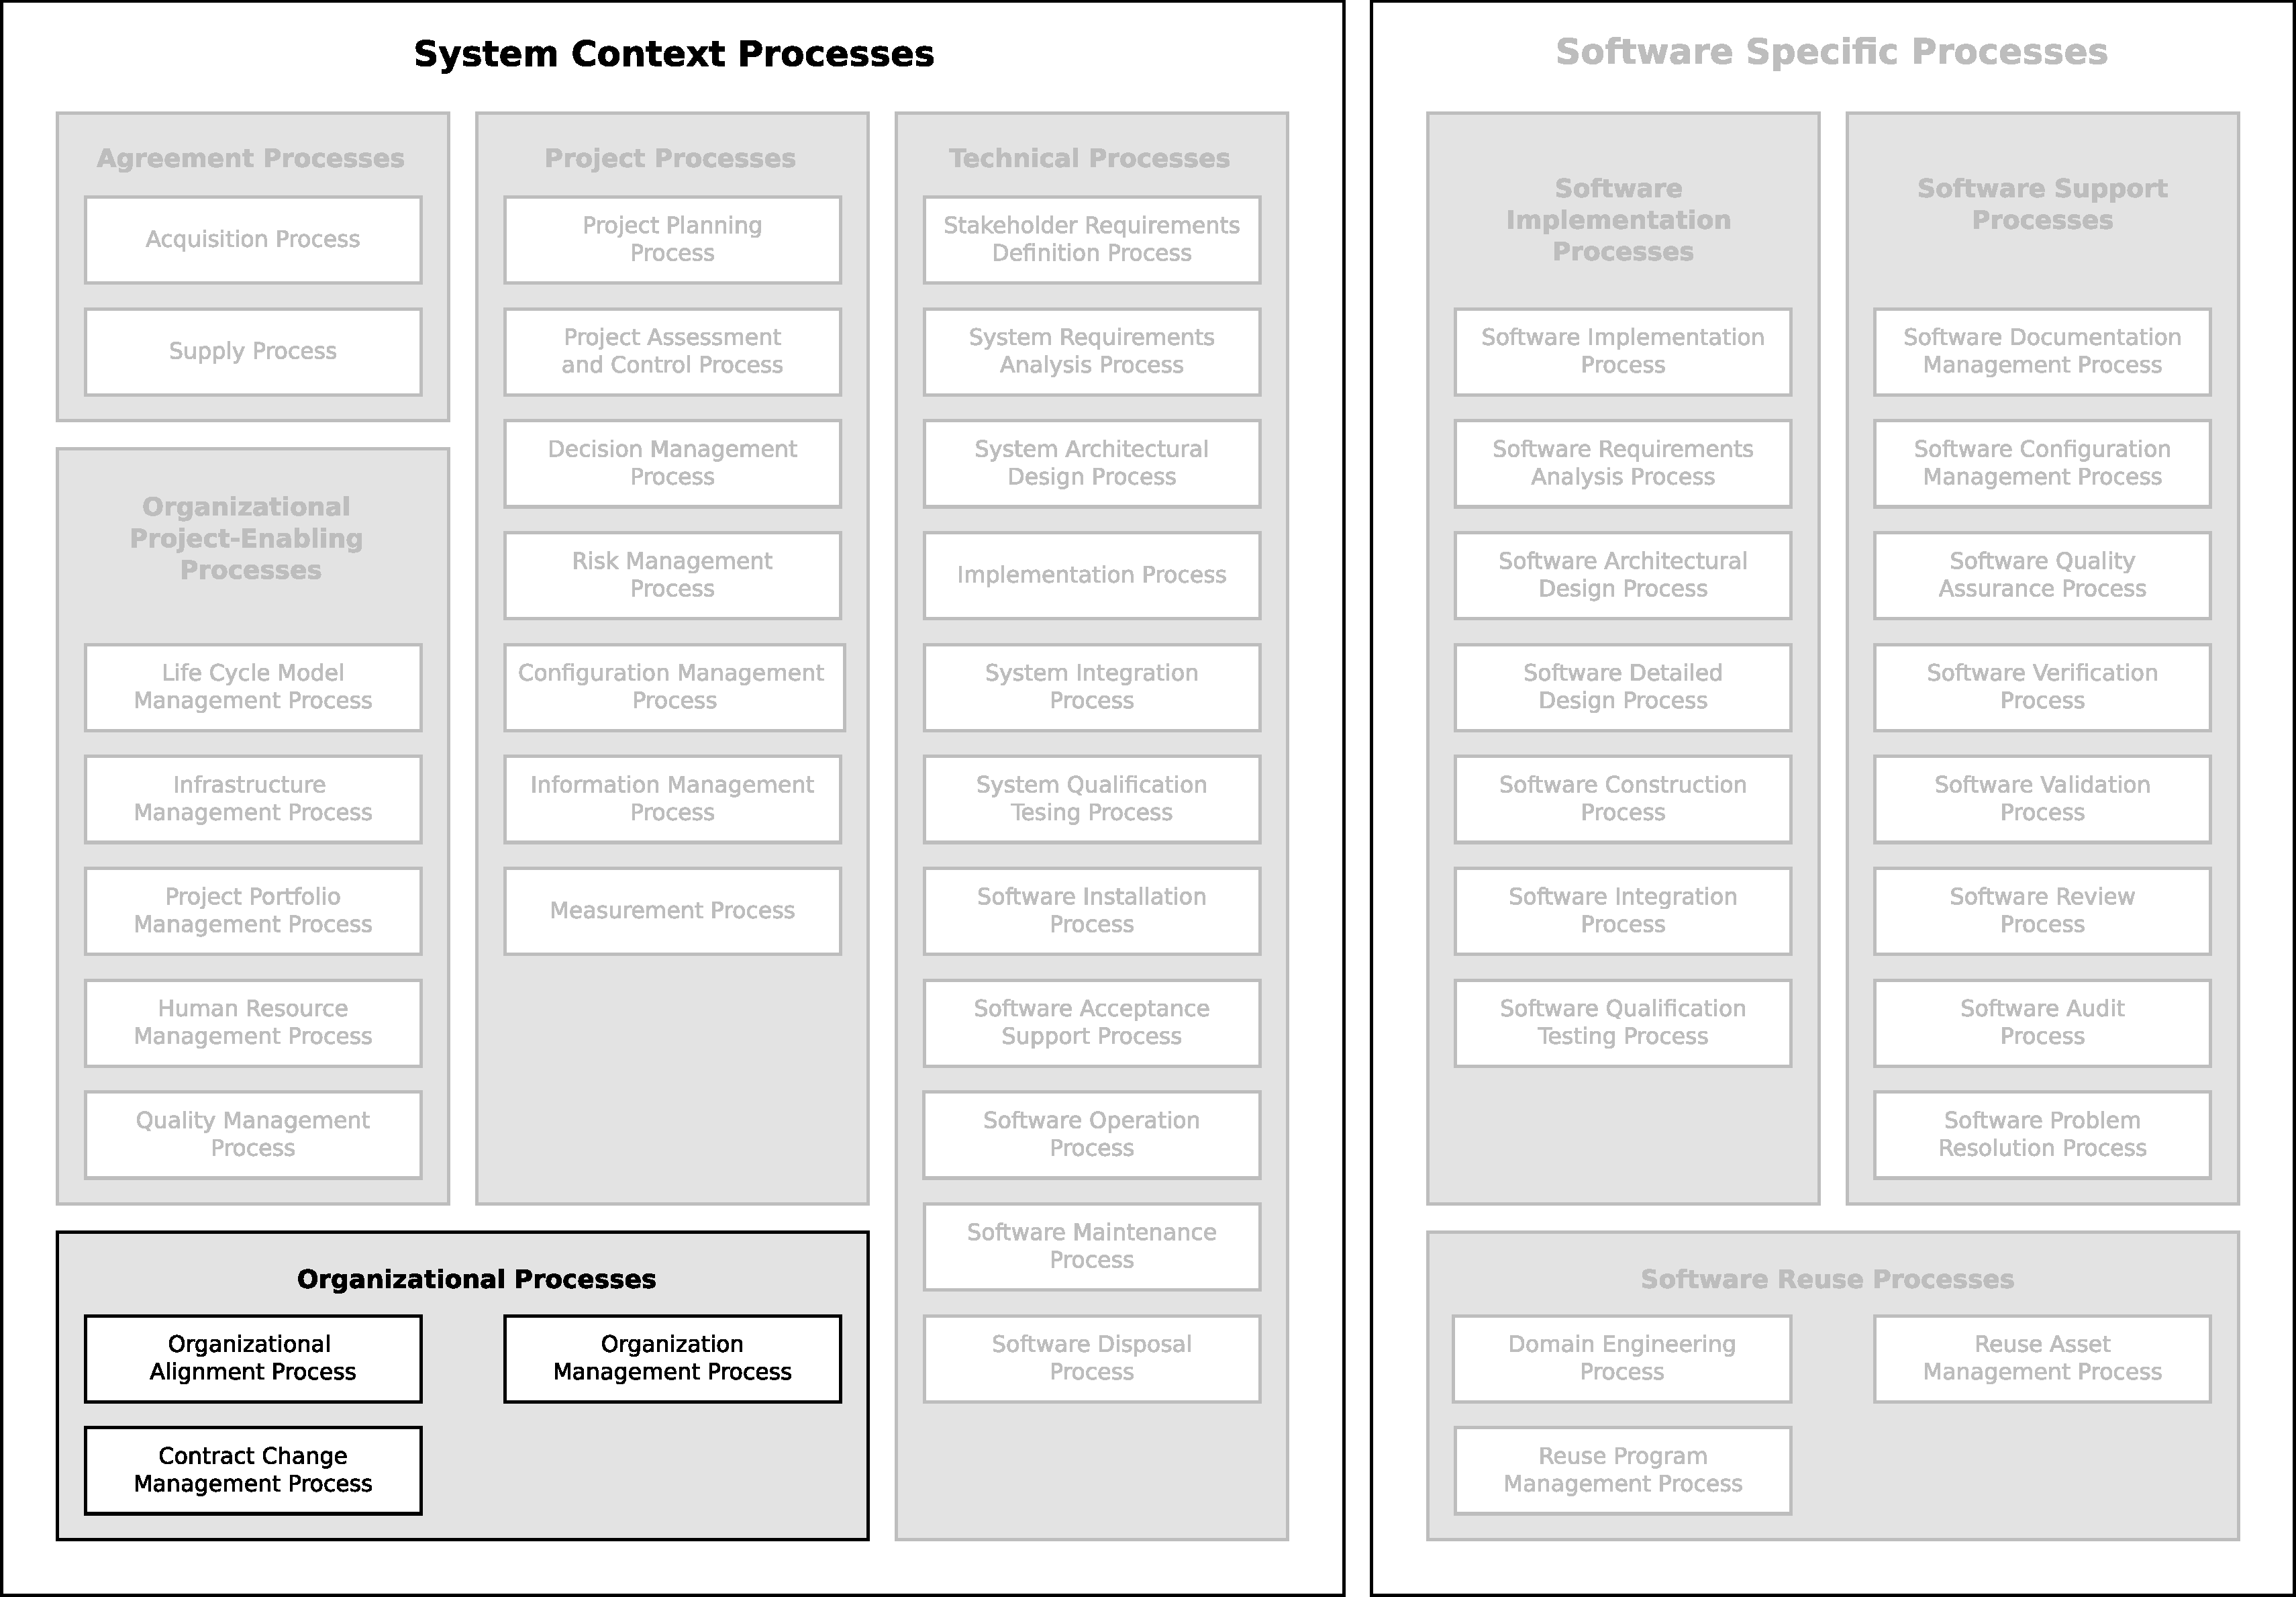
\includegraphics[width=15cm,keepaspectratio]{figures/life-cycle-process-groups-organizational-processes.pdf}
			\caption{Organizational Processes}
			\label{fig:organizational_processes}
		\end{figure}

		\begin{adjustwidth}{1em}{0pt}

			The processes within this section are considered highly useful to the management of an organization and its use and management of the processes within this standard.

			In this Section:

			\begin{compactitem}
			
				\item \ref{proc:organizational_alignment_process} - \nameref{proc:organizational_alignment_process}

				\item \ref{proc:organization_management_process} - \nameref{proc:organization_management_process}

				\item \ref{proc:contract_change_management_process} - \nameref{proc:contract_change_management_process}
			
			\end{compactitem}

		\end{adjustwidth}

		\newpage
		\subsubsection{ORGANIZATIONAL ALIGNMENT PROCESS\label{proc:organizational_alignment_process}}
		
			\subsubsubsection{PURPOSE}
			\begin{adjustwidth}{2em}{0pt}

				The purpose of the \nameref{proc:organizational_alignment_process} is to enable the software processes needed by the organization to provided software products and services, to be consistent with its goals. Within this context, goals are defined by the business' highest-order business objectives. 

			\end{adjustwidth}

			\subsubsubsection{OUTCOMES}
			\begin{adjustwidth}{2em}{0pt}

				\begin{compactitem}

					\item The organization's business goals are identified;

					\item The process framework is identified and defined that includes a set of software processes needed to achieve the business goals of the organization;
					
					\item A strategy is defined for process definition, implementation and improvement;
					
					\item Support is provided to enable this strategy;
					
					\item The organization's mission, core values, vision, goals and objectives is made known to all employees;
					
					\item Individuals in the organization share a common vision, culture, and understanding of the business goals to empower them to function effectively; and
					
					\item Everyone in the organization understands their role in achieving the goals of the business and is able to perform that role.
				
				\end{compactitem}

			\end{adjustwidth}

		\newpage
		\subsubsection{ORGANIZATION MANAGEMENT PROCESS\label{proc:organization_management_process}}

			\subsubsubsection{PURPOSE}
			\begin{adjustwidth}{2em}{0pt} 

				The purpose of the \nameref{proc:organization_management_process} is to establish and perform software management practices, during the performance of the processes needed for providing software products and services, that are consistent with the business goals of the organization.

				{\bf Note}: Although organizational operations in general have a much broader scope than that of software process, software processes are implemented in a business context and to be effective, require an appropriate organizational environment.

			\end{adjustwidth}

			\subsubsubsection{OUTCOMES}
			\begin{adjustwidth}{2em}{0pt} 

				\begin{compactitem}

					\item the organization will invest in the appropriate management infrastructure;

					\item the best practices are identified to support the implementation of effective organization and project management; and

					\item a basis for evaluating the achievement of organization business goals based on these management practices is provided.

				\end{compactitem}

			\end{adjustwidth}

		\newpage
		\subsubsection{CONTRACT CHANGE MANAGEMENT PROCESS\label{proc:contract_change_management_process}}

			\subsubsubsection{PURPOSE}
			\begin{adjustwidth}{2em}{0pt} 

				The purpose of the \nameref{proc:contract_change_management_process} is to develop the new contract contents as agreed by both the acquirer and the supplier when a change request affecting the agreed contract contents is proposed. 

				This process begins with a proposal of the change request by either the acquirer or the supplier and ends with the conclusion acceptable for both parties: withdrawal or overall/partial approval of the change request.

			\end{adjustwidth}

			\subsubsubsection{OUTCOMES}
			\begin{adjustwidth}{2em}{0pt} 

				\begin{compactitem}

					\item the change request to the contract is proposed explicitly and formally;

					\item the roles and responsibilities of both the acquirer and the supplier for the contract change management are established;

					\item the impact of the change request to the contract on the project plans, costs, benefits, quality and schedule is evaluated;

					\item the actions against the change request are taken to get agreement and satisfaction of both the acquirer and the supplier; and

					\item the result of each change request is made known to all affected parties.

				\end{compactitem}

			\end{adjustwidth}


	\newpage 
	\subsection{TECHNICAL PROCESSES\label{subsec:technical_processes}}

		\begin{figure}[h]
			\centering
			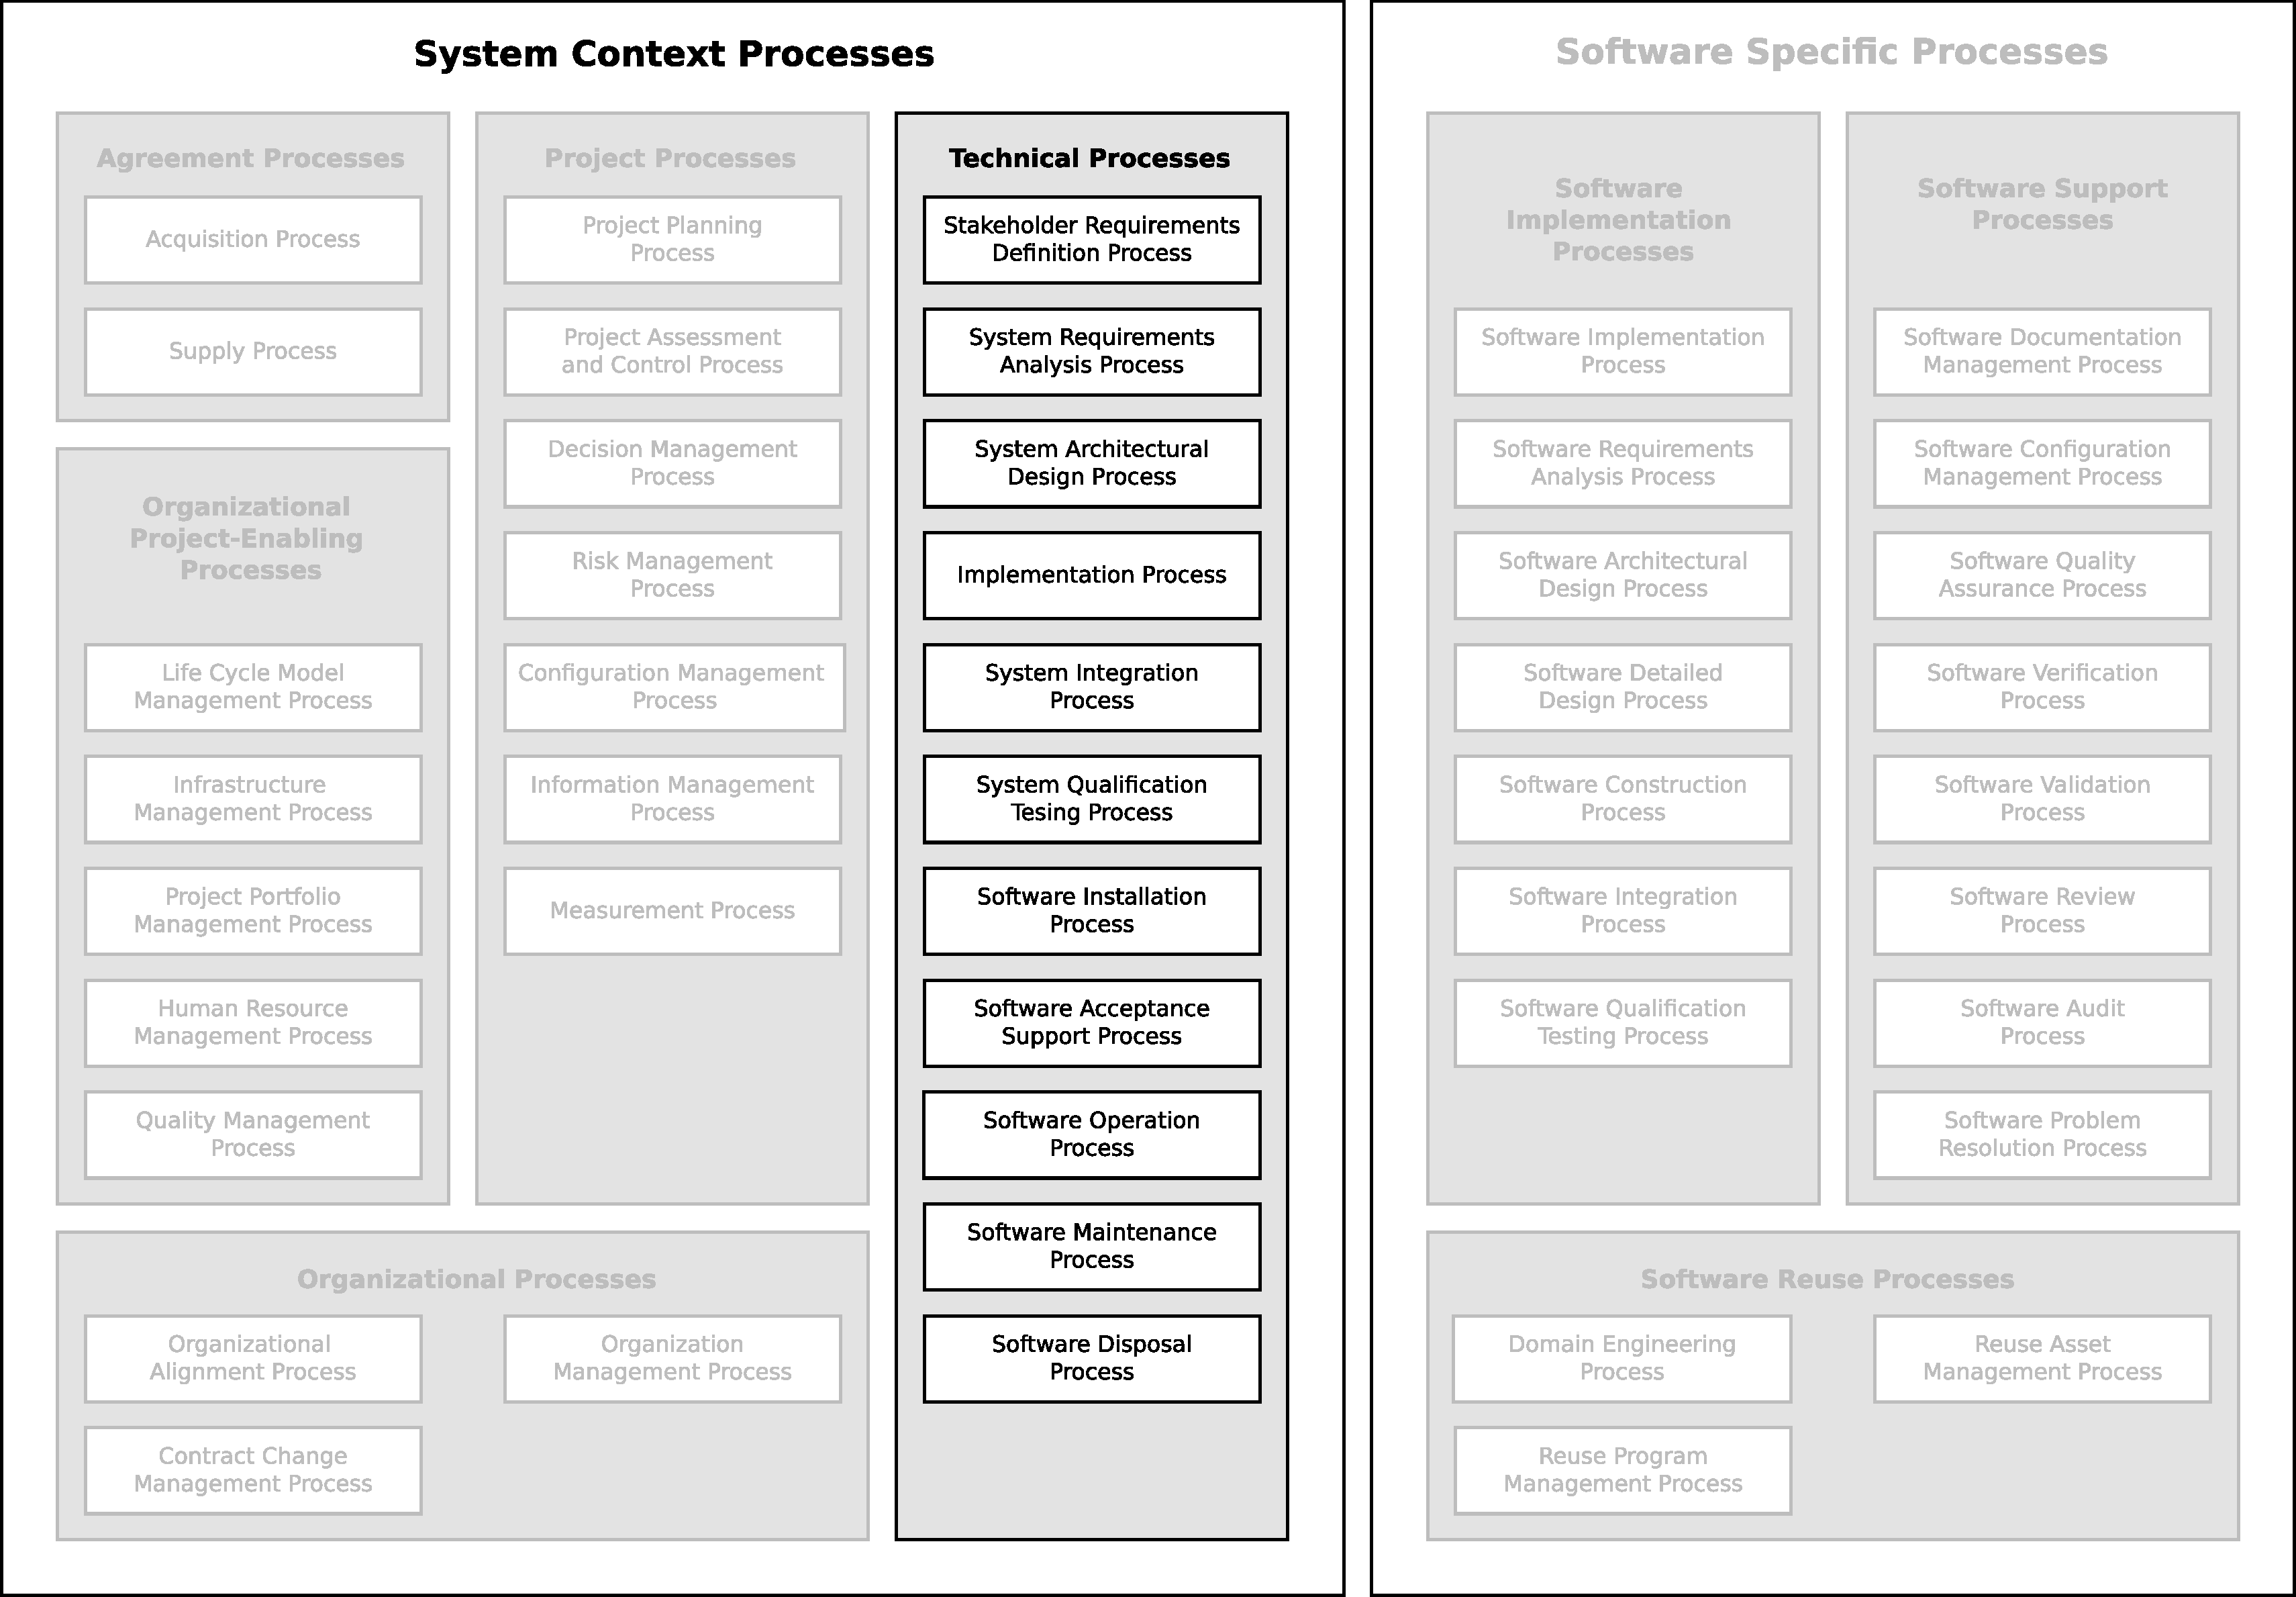
\includegraphics[width=15cm,keepaspectratio]{figures/life-cycle-process-groups-technical-processes.pdf}
			\caption{Technical Processes}
			\label{fig:technical_processes}
		\end{figure}

		\begin{adjustwidth}{1em}{0pt}

			The Technical Processes define the activities that enable organizational and project functions to optimize the benefits and reduce the risks that arise from technical decisions and actions. 

			These activities enable products and services to possess the timeliness and availability, the cost effectiveness, and the functionality, reliability, maintainability, producibility, usability and other qualities required by acquiring and supplying organizations. They also enable products and services to conform to the expectations or legislated requirements of society, including health, safety, security and environmental factors.

			\begin{compactitem}
			
				\item \ref{proc:stakeholder_requirements_definition_process} - \nameref{proc:stakeholder_requirements_definition_process}

				\item \ref{proc:system_requirements_analysis_process} - \nameref{proc:system_requirements_analysis_process}

				\item \ref{proc:system_architectural_design_process} - \nameref{proc:system_architectural_design_process}

				\item \ref{proc:implementation_process} - \nameref{proc:implementation_process}

				\item \ref{proc:system_integration_process} - \nameref{proc:system_integration_process}

				\item \ref{proc:system_qualification_testing_process} - \nameref{proc:system_qualification_testing_process}

				\item \ref{proc:software_installation_process} - \nameref{proc:software_installation_process}

				\item \ref{proc:software_acceptance_support_process} - \nameref{proc:software_acceptance_support_process}

				\item \ref{proc:software_operation_process} - \nameref{proc:software_operation_process}

				\item \ref{proc:software_maintenance_process} - \nameref{proc:software_maintenance_process}

				\item \ref{proc:software_disposal_process} - \nameref{proc:software_disposal_process}
			
			\end{compactitem}

		\end{adjustwidth}

		\newpage
		\subsubsection{STAKEHOLDER REQUIREMENTS DEFINITION PROCESS\label{proc:stakeholder_requirements_definition_process}}

			\subsubsubsection{PURPOSE}
			\begin{adjustwidth}{2em}{0pt} 
			
				The purpose of the \nameref{proc:stakeholder_requirements_definition_process} is to define the requirements for a system that can provide the services needed by users and other stakeholders in a defined environment.

				It identifies stakeholders, or stakeholder classes, involved with the system throughout its life cycle, and their needs and desires. It analyzes and transforms these into a common set of stakeholder requirements that express the intended interaction the system will have with its operational environment and that are the reference against which each resulting operational service is validated in order to confirm that the system fulfills needs.

			\end{adjustwidth}

			\subsubsubsection{OUTCOMES}
			\begin{adjustwidth}{2em}{0pt} 

				\begin{compactitem}

					\item the required characteristics and context of use of services are specified;

					\item the constraints on a system solution are defined;

					\item traceability of stakeholder requirements to stakeholders and their needs is achieved;

					\item the basis for defining the system requirements is described;

					\item the basis for validating the conformance of the services is defined; and

					\item a basis for negotiating and agreeing to supply a service or product is provided.

				\end{compactitem}

			\end{adjustwidth}

			\subsubsubsection{ACTIVITIES AND TASKS}
			\begin{adjustwidth}{2em}{0pt} 

				\begin{compactenum}

					\item {\bf Stakeholder Identification}:
					\begin{compactenum}

						\item The project shall identify the individual stakeholders or stakeholder classes who have a legitimate interest in the system throughout its life cycle.

					\end{compactenum}

					\item {\bf Requirements Identification}:
					\begin{compactenum}

						\item The project shall elicit stakeholder requirements.

						\item The project shall define the constraints on a system solution that are unavoidable consequences of existing agreements, management decisions and technical decisions.

						\item The project shall define a representative set of activity sequences to identify all required services that correspond to anticipated operational and support scenarios and environments.

						\item The project shall identify the interaction between users and the system, taking into the account human capabilities and skills limitations.

						\begin{compactenum}

							\item Physical, mental, and learned capabilities;

							\item Work place, environment and facilities, including other equipment in the context of use;

							\item Normal, unusual, and emergency conditions;

							\item Operator and user recruitment, training and culture.

						\end{compactenum}

						\item The project shall specify health, safety, security, environment and other stakeholder requirements and functions that relate to critical qualities and shall address possible adverse effects of use of the system on human health and safety.

					\end{compactenum}

					\item {\bf Requirements Evaluation}:
					\begin{compactenum}

						\item The project shall analyze the complete set of elicited requirements.

					\end{compactenum}

					\item {\bf Requirements Agreement}:
					\begin{compactenum}

						\item The project shall resolve requirements problems.

						\item The project shall feed back the analyzed requirements to applicable stakeholders to ensure that the needs and expectations have been adequately captured and expressed.

						\item The project shall establish with stakeholders that their requirements are expressed correctly.

					\end{compactenum}

					\item {\bf Requirements Recording}:

					\begin{compactenum}

						\item The project shall record the stakeholder requirements in a form suitable for requirements management through the life cycle and beyond.

						\item The project shall maintain stakeholder requirements traceability to the sources of stakeholder need.

					\end{compactenum}

				\end{compactenum}

			\end{adjustwidth}

		\newpage
		\subsubsection{SYSTEM REQUIREMENTS ANALYSIS PROCESS\label{proc:system_requirements_analysis_process}}

			\subsubsubsection{PURPOSE}
			\begin{adjustwidth}{2em}{0pt} 

				The purpose of \nameref{proc:system_requirements_analysis_process} is to transform the defined stakeholder requirements into a set of desired system technical requirements that will standard the design of the system.

			\end{adjustwidth}

			\subsubsubsection{OUTCOMES}
			\begin{adjustwidth}{2em}{0pt} 

				\begin{compactitem}

					\item a defined set of system functional and non-functional requirements describing the problem to be solved are established;

					\item the appropriate techniques are performed to optimize the preferred project solution;

					\item system requirements are analyzed for correctness and testability;

					\item the impact of the system requirements on the operating environment are understood;

					\item the requirements are prioritized, approved and updated as needed;

					\item consistency and traceability are established between the system requirements and the customer's requirements baseline;

					\item changes to the baseline are evaluated for cost, schedule and technical impact; and

					\item the system requirements are communicated to all affected parties and baselined.

				\end{compactitem}

			\end{adjustwidth}

			\subsubsubsection{ACTIVITIES AND TASKS}
			\begin{adjustwidth}{2em}{0pt} 

				\begin{compactenum}

					\item {\bf Requirements Specification}:

					\begin{compactenum}

						\item The specific intended use of the system to be developed shall be analyzed to specify system requirements. The system requirements specification shall describe: functions and capabilities of the system; business, organizational and user requirements; safety, security, human-factors engineering (ergonomics), interface, operations, and maintenance requirements; design constraints and qualification requirements. The system requirements specification shall be documented.

					\end{compactenum}

					\item {\bf Requirements Evaluation}:

					\begin{compactenum}

						\item The system requirements shall be evaluated considering the criteria listed below. The results of evaluations shall be documented.

						\begin{compactenum}

							\item Traceability to acquisition needs;

							\item Consistency with acquisition needs;

							\item Testability;

							\item Feasibility of system architectural design;

							\item Feasibility of operation and maintenance.

						\end{compactenum}

					\end{compactenum}

				\end{compactenum}

			\end{adjustwidth}

		\newpage
		\subsubsection{SYSTEM ARCHITECTURAL DESIGN PROCESS\label{proc:system_architectural_design_process}}
		
			\subsubsubsection{PURPOSE}
			\begin{adjustwidth}{2em}{0pt} 
				
				The purpose of the \nameref{proc:system_architectural_design_process} is to identify which system requirements should be allocated to which elements of the system.

			\end{adjustwidth}

			\subsubsubsection{OUTCOMES}
			\begin{adjustwidth}{2em}{0pt} 

				\begin{compactitem}

					\item a system architecture design is defined that identifies the elements of the system and meets the defined requirements;

					\item the system's functional and non-functional requirements are addressed;

					\item the requirements are allocated to the elements of the system;

					\item internal and external interfaces of each system element are defined;

					\item verification between the system requirements and the system architecture is performed;

					\item the requirements allocated to the system elements and their interfaces are traceable to the customer's requirements baseline;

					\item consistency and traceability between the system requirements and system architecture design is maintained; and

					\item the system requirements, the system architecture design, and their relationships are baselined and communicated to all affected parties;

					\item human factors and ergonomic knowledge and techniques are incorporated in system design; and

					\item human-centered design activities are identified and performed.

				\end{compactitem}

			\end{adjustwidth}

			\subsubsubsection{ACTIVITIES AND TASKS}
			\begin{adjustwidth}{2em}{0pt} 

				\begin{compactenum}

					\item {\bf Establishing Architecture}:
					\begin{compactenum}

						\item A top-level architecture of the system shall be established. The architecture shall identify items of hardware, software, and manual operations. It shall be ensured that all the system requirements are allocated among the items. Hardware configuration items, software configuration items, and manual operations shall be subsequently identified from these items. The system architecture and the system requirements allocated to the items shall be documented.

					\end{compactenum}

					\item {\bf Architectural Evaluation}:
					\begin{compactenum}

						\item The system architecture and the requirements for the items shall be evaluated considering the criteria listed below. The results of the evaluations shall be documented.

						\begin{compactenum}

							\item Traceability to the system requirements.

							\item Consistency with the system requirements.

							\item Appropriateness of design standards and methods used.

							\item Feasibility of the software items fulfilling their allocated requirements.

							\item Feasibility of operation and maintenance.

						\end{compactenum}

					\end{compactenum}

				\end{compactenum}

			\end{adjustwidth}

		\newpage
		\subsubsection{IMPLEMENTATION PROCESS\label{proc:implementation_process}}

			\subsubsubsection{PURPOSE}
			\begin{adjustwidth}{2em}{0pt} 
				
				The purpose of the \nameref{proc:implementation_process} is to realize a specified system element.

				{\bf Note}: This process is intentionally void of outcomes, activities, and tasks, as the implementation process to realize any given system element is contingent upon the context of that element. See \nameref{proc:software_implementation_process} for how the implementation process is defined for software, as an example. 

			\end{adjustwidth}

		\newpage
		\subsubsection{SYSTEM INTEGRATION PROCESS\label{proc:system_integration_process}}

			\subsubsubsection{PURPOSE}
			\begin{adjustwidth}{2em}{0pt} 

				The purpose of the \nameref{proc:system_integration_process} is to integrate the system elements (including software items, hardware items, manual operations, and other systems, as necessary) to produce a complete system that will satisfy the system design and the customers’ expectations expressed in the system requirements.

			\end{adjustwidth}


			\subsubsubsection{OUTCOMES}
			\begin{adjustwidth}{2em}{0pt} 

				\begin{compactitem}

					\item a strategy is developed to integrate the system according to the priorities of the system requirements;

					\item criteria are developed to verify compliance with the system requirements allocated to the system elements, including the interfaces between system elements;

					\item the system integration is verified using the defined criteria;

					\item a regression strategy is developed and applied for re-testing the system when changes are made;

					\item consistency and traceability are established between the system design and the integrated system elements;

					\item an integrated system is constructed that demonstrates compliance with the system design; and

					\item an integrated system is constructed that demonstrates that a complete set of usable deliverable system elements exists.

				\end{compactitem}

			\end{adjustwidth}

			\subsubsubsection{ACTIVITIES AND TASKS}
			\begin{adjustwidth}{2em}{0pt} 

				\begin{compactenum}

					\item {\bf Integration}:

					\begin{compactenum}

							\item The software configuration items shall be integrated, with hardware configuration items, manual operations, and other systems as necessary, into the system. The aggregates shall be tested, as they are developed, against their requirements. The integration and the test results shall be documented.

					\end{compactenum}

					\item {\bf Test Readiness}:

					\begin{compactenum}

							\item For each qualification requirement of the system, a set of tests, test cases (inputs, outputs, test criteria), and test procedures for conducting System Qualification Testing shall be developed and documented. The developer shall ensure that the integrated system is ready for System Qualification Testing.

							\item The integrated system shall be evaluated considering the criteria listed below. The results of the evaluations shall be documented.

							\begin{compactenum}

								\item Test coverage of system requirements.

								\item Appropriateness of test methods and standards used.

								\item Conformance to expected results.

								\item Feasibility of system qualification testing.

								\item Feasibility of operation and maintenance.

							\end{compactenum}

					\end{compactenum}

				\end{compactenum}

			\end{adjustwidth}

		\newpage
		\subsubsection{SYSTEM QUALIFICATION TESTING PROCESS\label{proc:system_qualification_testing_process}}

			\subsubsubsection{PURPOSE}
			\begin{adjustwidth}{2em}{0pt} 

				The purpose of the \nameref{proc:system_qualification_testing_process} is to ensure that the implementation of each system requirement is tested for compliance and that the system is ready for delivery.

			\end{adjustwidth}

			\subsubsubsection{OUTCOMES}
			\begin{adjustwidth}{2em}{0pt} 

				\begin{compactitem}

					\item criteria for evaluating compliance with system requirements are developed;

					\item the integrated system is tested using the defined criteria;

					\item test results are recorded; and

					\item readiness of the system for delivery is assured.

				\end{compactitem}

			\end{adjustwidth}

			\subsubsubsection{ACTIVITIES AND TASKS}
			\begin{adjustwidth}{2em}{0pt} 

				\begin{compactenum}

					\item {\bf Qualification Testing}:

					\begin{compactenum}

						\item System qualification testing shall be conducted in accordance with the qualification requirements specified for the system. 

						\item It shall be ensured that the implementation of each system requirement is tested for compliance and that the system is ready for delivery.

						\item The qualification testing results shall be documented.

						\item The system shall be evaluated considering the criteria listed below. evaluations shall be documented.

						\begin{compactenum}

							\item Test coverage of system requirements;

							\item Conformance to expected results;

							\item Feasibility of operation and maintenance.

						\end{compactenum}

						\item The developer shall support audit(s) in accordance with \nameref{proc:software_audit_process}. The results of the audit(s) shall be documented.

						\item Upon successful completion of the audit(s), if conducted, the developer shall update and prepare the deliverable software product for Software Installation and Software Acceptance Support.

					\end{compactenum}

				\end{compactenum}

			\end{adjustwidth}

		\newpage
		\subsubsection{SOFTWARE INSTALLATION PROCESS\label{proc:software_installation_process}}

			\subsubsubsection{PURPOSE}
			\begin{adjustwidth}{2em}{0pt} 

				The purpose of the \nameref{proc:software_installation_process} is to install the software product that meets the agreed requirements in the target environment.

			\end{adjustwidth}

			\subsubsubsection{OUTCOMES}
			\begin{adjustwidth}{2em}{0pt} 

				\begin{compactitem}

					\item a software installation strategy is developed;

					\item criteria for software installation are developed that demonstrate compliance with the software installation requirements;

					\item the software product is installed in the target environment; and

					\item readiness of the software product for use in its intended environment is assured.

				\end{compactitem}

			\end{adjustwidth}

			\subsubsubsection{ACTIVITIES AND TASKS}
			\begin{adjustwidth}{2em}{0pt} 

				\begin{compactenum}

					\item {\bf Software Installation}:

					\begin{compactenum}

						\item The implementer shall develop a plan to install the software product in the target environment as designated in the contract. The resources and information necessary to install the software product shall be determined and be available. As specified in the contract, the implementer shall assist the acquirer with the set-up activities.  Where the installed software product is replacing an existing system, the implementer shall support any parallel running activities that are required by contract. The installation plan shall be documented.

						\item The developer shall install the software product in accordance with the installation plan. It shall be ensured that the software code and databases initialize, execute, and terminate as specified in the contract. The installation events and results shall be documented.

					\end{compactenum}

				\end{compactenum}

			\end{adjustwidth}

		\newpage
		\subsubsection{SOFTWARE ACCEPTANCE SUPPORT PROCESS\label{proc:software_acceptance_support_process}}

			\subsubsubsection{PURPOSE}
			\begin{adjustwidth}{2em}{0pt} 

				The purpose of the \nameref{proc:software_acceptance_support_process} is to assist the acquirer to achieve confidence that the product meets requirements.

			\end{adjustwidth}

			\subsubsubsection{OUTCOMES}
			\begin{adjustwidth}{2em}{0pt} 

				\begin{compactitem}

					\item the product is completed and delivered to the acquirer;

					\item acquirer acceptance tests and reviews are supported;

					\item the product is put into operation in the customers’ environment; and

					\item problems detected during acceptance are identified and communicated to those responsible for resolution.

				\end{compactitem}

			\end{adjustwidth}

			\subsubsubsection{ACTIVITIES AND TASKS}
			\begin{adjustwidth}{2em}{0pt} 

				\begin{compactenum}

					\item {\bf Software Acceptance Support}:

					\begin{compactenum}

						\item The developer shall support the acquirer's acceptance review and testing of the software product. Acceptance review and testing shall consider the results of the \nameref{proc:software_review_process}, \nameref{proc:software_audit_process}, \nameref{proc:software_qualification_testing_process}, and \nameref{proc:system_qualification_testing_process} (if performed) processes. The results of the acceptance review and testing shall be documented.

						\item The developer shall complete and deliver the software product as specified in the contract.

						\item The developer shall provide initial and continuing training and support to the acquirer as specified in the contract.

					\end{compactenum}

				\end{compactenum}

			\end{adjustwidth}

		\newpage
		\subsubsection{SOFTWARE OPERATION PROCESS\label{proc:software_operation_process}}

			\subsubsubsection{PURPOSE}
			\begin{adjustwidth}{2em}{0pt} 
				
				The purpose of the \nameref{proc:software_operation_process} is to operate the software product in its intended environment and to provide support to the customers of the software product.

			\end{adjustwidth}

			\subsubsubsection{OUTCOMES}
			\begin{adjustwidth}{2em}{0pt} 

				\begin{compactitem}

					\item an operation strategy is defined;

					\item conditions for correct operation of the software in its intended environment are identified and evaluated;

					\item the software is tested and determined to operate in its intended environment;

					\item the software is operated in its intended environment; and

					\item assistance and consultation is provided to the customers of the software product in accordance with the agreement.

				\end{compactitem}

			\end{adjustwidth}

			\subsubsubsection{ACTIVITIES AND TASKS}
			\begin{adjustwidth}{2em}{0pt} 

				\begin{compactenum}

					\item {\bf Preparation for Operation}:

					\begin{compactenum}

						\item The operator shall develop a plan and set operational standards for performing the activities and tasks of this process. The plan shall be documented and executed.

						\item The operator shall establish procedures for receiving, recording, resolving, tracking problems, and providing feedback. Whenever problems are encountered, they shall be recorded and entered into the \nameref{proc:software_problem_resolution_process}.

						\item The operator shall establish procedures for testing the software product in its operation environment, for entering problem reports and modification requests to the \nameref{proc:software_maintenance_process}, and for releasing the software product for operational use.

					\end{compactenum}

					\item {\bf Operation Activation and Check-out}:

					\begin{compactenum}

						\item For each release of the software product, the operator shall perform operational testing, and, on satisfying the specified criteria, release the software product for operational use.

						\item The operator shall ensure that the software code and databases initialize, execute, and terminate as described in the plan.

						\item The operator shall activate the system in its intended operational situation to deliver instances of service or continuous service according to its intended purpose.

					\end{compactenum}

					\item {\bf Operational Use}:

					\begin{compactenum}

						\item The system shall be operated in its intended environment according to the user documentation.

					\end{compactenum}

					\item {\bf Customer Support}:

					\begin{compactenum}

						\item The operator shall provide assistance and consultation to the users as requested. These requests and subsequent actions shall be recorded and monitored.

						\item The operator shall forward user requests, as necessary, to the \nameref{proc:software_maintenance_process} for resolution. These requests shall be addressed and the actions that are planned and taken shall be reported to the originators of the requests. All resolutions shall be monitored to conclusion.

					\end{compactenum}

					\item {\bf Operational Problem Resolution}:

					\begin{compactenum}

						\item The operator shall forward identified problems to the Software Problem Resolution Process for resolution.

						\item If a reported problem has a temporary work-around before a permanent solution can be released, the originator of the problem report shall be given the option to use it. Permanent corrections, releases that include previously omitted functions or features, and system improvements shall be applied to the operational software product using the \nameref{proc:software_maintenance_process}.

					\end{compactenum}

				\end{compactenum}

			\end{adjustwidth}

		\newpage
		\subsubsection{SOFTWARE MAINTENANCE PROCESS\label{proc:software_maintenance_process}}

			\subsubsubsection{PURPOSE}
			\begin{adjustwidth}{2em}{0pt}  

				The purpose of the \nameref{proc:software_maintenance_process} is to provide cost-effective support to a delivered software product.

				{\bf Note}: Pre-delivery Software Maintenance activities include planning for post-delivery operations, supportability, and logistics determination. Post-delivery activities include software modification and operational support, such as training or operating a help desk.

			\end{adjustwidth}

			\subsubsubsection{OUTCOMES}
			\begin{adjustwidth}{2em}{0pt} 

				\begin{compactitem}

					\item a maintenance strategy is developed to manage modification and migration of products according to the release strategy;

					\item the impact of changes to the existing system on organization, operations or interfaces are identified;

					\item affected system and software documentation is updated as needed;

					\item modified products are developed with associated tests that demonstrate that requirements are not compromised;

					\item product upgrades are migrated to the customer’s environment; and

					\item the system software modification is communicated to all affected parties.

				\end{compactitem}

			\end{adjustwidth}

			\subsubsubsection{ACTIVITIES AND TASKS}
			\begin{adjustwidth}{2em}{0pt} 

				\begin{compactenum}

					\item {\bf Process Implementation}:

					\begin{compactenum}

						\item The maintainer shall develop, document, and execute plans and procedures for conducting the activities and tasks of the Software Maintenance Process.

						\item The maintainer shall establish procedures for receiving, recording, and tracking problem reports and modification requests from the users and providing feedback to the users. Whenever problems are encountered, they shall be recorded and entered into the \nameref{proc:software_problem_resolution_process}.

						\item The maintainer shall implement (or establish organizational interface with) the \nameref{proc:configuration_management_process} for managing modifications to the existing system.

					\end{compactenum}


					\item {\bf Problem and Modification Analysis}:

					\begin{compactenum}

						\item The maintainer shall analyze the problem report or modification request for its impact on the organization, the existing system, and the interfacing systems for the following:

						\begin{compactenum}

							\item Type; for example, corrective, improvement, preventive, or adaptive to new environment;

							\item Scope; for example, size of modification, cost involved, time to modify;

							\item Criticality; for example, impact on performance, safety, or security.

						\end{compactenum}

						\item The maintainer shall replicate or verify the problem.

						\item The maintainer shall document the problem/modification request, the analysis results, and implementation options.

						\item The maintainer shall obtain approval for the selected modification option as specified in the contract. 

					\end{compactenum}


					\item {\bf Modification Implementation}:

					\begin{compactenum}

						\item The maintainer shall conduct analysis and determine which documentation, software units, and versions thereof need to be modified. These shall be documented.

						\item The maintainer shall enter the \nameref{subsec:technical_processes} to implement the modifications. The requirements of the Technical Processes shall be supplemented as follows:

						\item Test and evaluation criteria for testing and evaluating the modified and the unmodified parts (software units, components, and configuration items) of the system shall be defined and documented.

						\item The complete and correct implementation of the new and modified requirements shall be ensured. It also shall be ensured that the original, unmodified requirements were not affected. The test results shall be documented.

					\end{compactenum}

					\item {\bf Maintenance Review/Acceptance}:

					\begin{compactenum}

						\item The maintainer shall conduct review(s) with the organization authorizing the modification to determine the integrity of the modified system.

						\item The maintainer shall obtain approval for the satisfactory completion of the modification as specified in the contract.

					\end{compactenum}

					\item {\bf Migration}:

					\begin{compactenum}

						\item If a system or software product (including data) is migrated from an old to a new operational environment, it shall be ensured that any software product or data produced or modified during migration is in accordance with this standard.

						\item A migration plan shall be developed, documented, and executed. The planning activities shall include users. Items included in the plan shall include the following:

						\begin{compactenum}

							\item Requirements analysis and definition of migration.

							\item Development of migration tools.

							\item Conversion of software product and data.

							\item Migration execution.

							\item Migration verification.

							\item Support for the old environment in the future.

						\end{compactenum}

						\item Users shall be given notification of the migration plans and activities. Notifications shall include the following:

						\begin{compactenum}

							\item Statement of why the old environment is no longer to be supported.

							\item Description of the new environment with its date of availability.

							\item Description of other support options available, if any, once support for the old environment has been removed.

						\end{compactenum}


						\item Parallel operations of the old and new environments may be conducted for smooth transition to the new environment. During this period, necessary training shall be provided as specified in the contract.

						\item When the scheduled migration arrives, notification shall be sent to all concerned. Associated old environment documentation, logs, and code should be placed in archives.

						\item A post-operation review shall be performed to assess the impact of changing to the new environment. The results of the review shall be sent to the appropriate authorities for information, guidance, and action.

						\item Data used by or associated with the old environment shall be accessible in accordance with the contract requirements for data protection and audit applicable to the data.

					\end{compactenum}

				\end{compactenum}

			\end{adjustwidth}

		\newpage
		\subsubsection{SOFTWARE DISPOSAL PROCESS\label{proc:software_disposal_process}}

			\subsubsubsection{PURPOSE}
			\begin{adjustwidth}{2em}{0pt} 

				The purpose of the \nameref{proc:software_disposal_process} is to end the existence of a system's software entity. This process ends active support by the operation and maintenance organization, or deactivates, disassembles and removes the affected software products, consigning them to a final condition and leaving the environment in an acceptable condition. 

				This process destroys or stores system software elements and related products in a sound manner, in accordance with legislation, agreements, organizational constraints and stakeholder requirements. Where required, it maintains records that may be monitored.
				
				{\bf Note}: The objective is to retire a system's existing software products or services while preserving the integrity of organizational operations.
			
			\end{adjustwidth}

			\subsubsubsection{OUTCOMES}
			\begin{adjustwidth}{2em}{0pt} 

				\begin{compactitem}

					\item a software disposal strategy is defined;

					\item disposal constraints are provided as inputs to requirements;

					\item the system's software elements are destroyed or stored;

					\item the environment is left in an agreed-upon state; and

					\item records allowing knowledge retention of disposal actions and any analysis of long-term impacts are available.

				\end{compactitem}

			\end{adjustwidth}

			\subsubsubsection{ACTIVITIES AND TASKS}
			\begin{adjustwidth}{2em}{0pt} 

				\begin{compactenum}

					\item {\bf Software Disposal Planning}:

					\begin{compactenum}

						\item A software disposal strategy is defined and documented. A plan to remove active support by the operation and maintenance organizations shall be developed and documented. The planning activities shall include users. The software disposal plan shall address the items listed below:

						\begin{compactenum}

							\item Cessation of full or partial support after a certain period of time.

							\item Archiving of the software product and its associated documentation.

							\item Responsibility for any future residual support issues.

							\item Transition to any new software product, if applicable.

							\item Accessibility of archive copies of data.

						\end{compactenum}

					\end{compactenum}

					\item {\bf Software Disposal Execution}:

					\begin{compactenum}

						\item The software disposal plan shall be executed.

						\item Users shall be given notification of the plans and activities for the retirement of software products and services. Notifications shall include the following:

						\begin{compactenum}

							\item Description of any replacement or upgrade with its date of availability.

							\item Statement of why the software product is no longer to be supported.

							\item Description of other support options available, once support has been removed.

						\end{compactenum}

						\item Parallel operations of the retiring and any new software product should be conducted for smooth transition to the new system. During this period, user training shall be provided as specified in the contract.

						\item When the scheduled retirement arrives, notification shall be sent to all concerned. All associated development documentation, logs, and code should be placed in archives, when appropriate.

						\item Data used by, or associated with, the retired software product shall be accessible in accordance with the contract requirements for data protection and audit applicable to the data.

					\end{compactenum}

				\end{compactenum}

			\end{adjustwidth}